\documentclass[11pt,a4paper]{report}

%==============================
% Encoding & Typography
%==============================

\usepackage[T1]{fontenc}
\usepackage[utf8]{inputenc}      % Not strictly necessary with modern LaTeX
\usepackage{lmodern}
\usepackage{svg}
\usepackage{microtype}
\microtypesetup{nopatch=footnote}  % suppress patch failure warning on some engines
\usepackage{csquotes}

% Silence siunitx's physics-package warning while keeping the RenewCommandCopy fix.
\ExplSyntaxOn
\msg_redirect_name:nnn { siunitx } { physics-pkg } { none }
\ExplSyntaxOff

%==============================
% Mathematics
%==============================

\usepackage{amsmath}
\usepackage{amssymb}
\usepackage{amsfonts}
\usepackage{amsthm}
\usepackage{mathtools}
\usepackage{bm}                  % Bold math symbols
\usepackage{braket}              % Alternative bra-ket notation
\usepackage{siunitx}
\usepackage{physics}             % \ket \bra \dv \pdv etc. (loads after siunitx to avoid its physics warning)
\AtBeginDocument{\RenewCommandCopy\qty\SI}  % keep siunitx's \qty despite physics package

%==============================
% Graphics
%==============================

\usepackage{graphicx}
\usepackage{xcolor}
\usepackage{float}
\usepackage{subcaption}
\usepackage{wrapfig}
\usepackage{tikz}
\usetikzlibrary{
    positioning,
    arrows.meta,
    calc,
    shapes,
    decorations.pathreplacing,
    fit
}

%==============================
% Tables
%==============================

\usepackage{array}
\usepackage{booktabs}
\usepackage{multirow}
\usepackage{longtable}
\usepackage{tabularx}
\usepackage{threeparttable}
\usepackage{makecell}

%==============================
% Algorithms
%==============================

\usepackage[ruled,vlined,linesnumbered]{algorithm2e}

%==============================
% Source code
%==============================

\usepackage{listings}

\lstset{
    basicstyle=\ttfamily\small,
    numbers=left,
    frame=single,
    breaklines=true,
    tabsize=4
}

%==============================
% References
%==============================

\usepackage[
    backend=biber,
    style=ieee,
    doi=true,
    url=false,
    isbn=false
]{biblatex}

% Suppress "(visited on ...)" access-date clauses from every @online-type
% bibliography entry (the ieee style prints these whenever urlyear/month/day
% are set, regardless of the url=false option above), without editing every
% urldate field in references.bib.
\AtEveryBibitem{\clearfield{urlday}\clearfield{urlmonth}\clearfield{urlyear}}

% standard.bbx only quotes titles for [article,inbook,incollection,
% inproceedings,patent,thesis,unpublished]; @misc falls back to italics with
% no quotes. Add @misc so it matches the same quoted-title style as the rest
% of the bibliography (e.g. the ITUT2024Cable entry).
\DeclareFieldFormat[misc]{title}{\mkbibquote{#1\isdot}}

\addbibresource{bibliography/references.bib}

%==============================
% Hyperlinks
%==============================

\usepackage{hyperref}
\usepackage{bookmark}  % generate PDF bookmarks in one pass
\usepackage[nameinlink]{cleveref}

\hypersetup{
    colorlinks=true,
    linkcolor=blue,
    citecolor=blue,
    urlcolor=blue,
    pdfauthor={Eliott FLECHTNER},
    pdftitle={Master Thesis}
}

%==============================
% Page layout
%==============================

\usepackage[a4paper,margin=2.5cm]{geometry}

\usepackage{setspace}
\onehalfspacing

\usepackage{fancyhdr}
\pagestyle{fancy}

%==============================
% Appendix
%==============================

\usepackage[toc,page]{appendix}

%==============================
% Lists
%==============================

\usepackage{enumitem}

%==============================
% Misc
%==============================

\usepackage{comment}
\usepackage{xspace}
\usepackage{url}

%==============================
% Acronyms
%==============================

\usepackage[acronym]{glossaries}

%==============================
% PDF inclusion
%==============================

\usepackage{pdfpages}
% Red marker for places that need a fix or clarification, and are likely wrong.
% For example, a formula that is known to be incorrect or a figure that is
% known to be misleading.
\newcommand{\TODO}[1]{\textcolor{red}{TODO: #1}}

% Orange marker for places that need a fix or clarification, but are not
% necessarily wrong. For example, a section that is not yet fully written or
% a figure that is not yet finalized.
\newcommand{\TOFIX}[1]{\textcolor{orange}{TOFIX: #1}}

% Dark blue marker for places that need a citation to external work
% (not yet in references.bib, or not yet decided which source to use).
\newcommand{\TOCITE}[1]{\textcolor{tocite}{[TO CITE: #1]}}

%% ==============================
% Math operators
\DeclareMathOperator{\Span}{Span}
\DeclareMathOperator*{\argmax}{arg\,max}
\DeclareMathOperator*{\argmin}{arg\,min}
%==============================
% Colours
%==============================
\definecolor{thesisblue}{RGB}{0,51,181}  % {0,51,102} = dark navy -- professional in print & screen
\definecolor{titlerule}{RGB}{80,80,80}     % soft dark-grey rule on titlepage
\definecolor{contentsblack}{RGB}{0,0,0}    % pure black for table of contents links
\definecolor{tocite}{RGB}{21,67,148}

% DAG node colours (match schedule/visualize.py _NODE_STYLE)
\definecolor{dagGen}{HTML}{AED6F1}        % light blue -- GenNode
\definecolor{dagJoin}{HTML}{F5B041}       % orange     -- JoinNode
\definecolor{dagSwap}{HTML}{82E0AA}       % green      -- SwapNode
\definecolor{dagPurify}{HTML}{C39BD3}     % purple     -- PurifyNode
\definecolor{dagIdle}{HTML}{D5D8DC}       % grey       -- IdleNode
\definecolor{dagHerald}{HTML}{F7DC6F}     % yellow     -- HeraldNode
\definecolor{dagRoot}{HTML}{F1948A}       % red        -- PauliCorrectNode
% Tiny filled square used as a colour swatch in node-type legends
\newcommand{\cswatch}[1]{\textcolor{#1}{\rule{0.85em}{0.85em}}}

% Figure colors
\definecolor{copyAblue}{RGB}{31,119,180}
\definecolor{copyBred}{RGB}{214,39,40}

%==============================
% Hyperlink colours
%==============================
\hypersetup{
    colorlinks=true,
    linkcolor=thesisblue,
    citecolor=thesisblue,
    urlcolor=thesisblue
}

%==============================
% Abstract (override report.cls which wraps in titlepage and resets \thepage)
%==============================
\renewenvironment{abstract}{%
  \chapter*{\abstractname}%
  \addcontentsline{toc}{chapter}{\abstractname}%
}{%
}

%==============================
% Running headers & footers (fancyhdr)
%==============================
\pagestyle{fancy}
\fancyhf{}
% Left header: chapter title (lower-case, no extra uppercase)
\fancyhead[L]{\small\nouppercase{\leftmark}}
% Right header: page number
\fancyhead[R]{\small\thepage}
\renewcommand{\headrulewidth}{0.4pt}
\renewcommand{\footrulewidth}{0.3pt}

% Footer: empty (logos belong on title page only)
\renewcommand{\footrulewidth}{0pt}

% Chapter-opening pages (plain style): page number centred, no rule
\fancypagestyle{plain}{%
  \fancyhf{}%
  \fancyfoot[C]{\small\thepage}%
  \renewcommand{\headrulewidth}{0pt}%
  \renewcommand{\footrulewidth}{0pt}%
}

%==============================
% Chapter Spacing Reductions
%==============================
\makeatletter
\def\@makechapterhead#1{%
  \vspace*{10\p@}% % Reduced top space (default: 50)
  {\parindent \z@ \raggedright \normalfont
    \ifnum \c@secnumdepth >\m@ne
        \huge\bfseries \@chapapp\ \thechapter
        \par\nobreak
        \vskip 8\p@
    \fi
    \interlinepenalty\@M
    \Huge \bfseries #1\par\nobreak
    \vskip 15\p@ % Space after chapter title (default: 40)
  }}
\def\@makeschapterhead#1{%
  \vspace*{10\p@}% % Reduced top space (default: 50)
  {\parindent \z@ \raggedright
    \normalfont
    \interlinepenalty\@M
    \Huge \bfseries #1\par\nobreak
    \vskip 25\p@ % Space after chapter title (default: 40)
  }}
\makeatother

%==============================
% Section spacing (titlesec's [compact] option is quite tight; nudge
% \section/\subsection spacing up slightly without abandoning compact mode)
%==============================
\titlespacing*{\section}{0pt}{2.2ex plus 0.3ex minus 0.2ex}{1.2ex plus 0.2ex}
\titlespacing*{\subsection}{0pt}{1.8ex plus 0.3ex minus 0.2ex}{1.0ex plus 0.2ex}
\newacronym{bsm}{BSM}{Bell-state measurement}
\newacronym{dag}{DAG}{directed acyclic graph}
\newacronym{rgs}{RGS}{repeater graph state}
\newacronym{rgss}{RGSS}{repeater graph state source}
\newacronym{absa}{ABSA}{advanced Bell-state analyser}
\newacronym{hrgs}{HRGS}{half-RGS}
% Notation glossary entries (type=notation inside key-value list).
% Preamble: % Notation glossary entries (type=notation inside key-value list).
% Preamble: % Notation glossary entries (type=notation inside key-value list).
% Preamble: \input{sections/notation} defines these entries.
% Body: \glsaddall[types={notation}] + \printglossary[type=notation,...] prints them.

% Network Configuration
\newglossaryentry{nc-N}{type=notation,
  name={$N$},
  description={Number of hops; an $N$-hop chain has $N+1$ stations $0,\dots,N$},
  sort={aN}}
\newglossaryentry{nc-calN}{type=notation,
  name={$\mathcal{N}$, $\mathcal{N}_{\mathrm{ref}}$},
  description={Network configuration; $\mathcal{N}_{\mathrm{ref}}$ is the reference configuration from the Integrating paper},
  sort={aNcal}}
\newglossaryentry{nc-ell}{type=notation,
  name={$\ell_i$},
  description={Length (km) of hop $i$},
  sort={aell}}
\newglossaryentry{nc-ed}{type=notation,
  name={$e_d$},
  description={Outer-qubit depolarizing rate per hop (photon-transmission error)},
  sort={aed}}
\newglossaryentry{nc-ki}{type=notation,
  name={$k_i$},
  description={Number of redundant BSM arms provisioned at hop $i$},
  sort={aki}}
\newglossaryentry{nc-gamma}{type=notation,
  name={$\gamma$},
  description={Memory dephasing rate; coherence time $T_2 = 1/\gamma$},
  sort={agamma}}
\newglossaryentry{nc-c}{type=notation,
  name={$c$},
  description={Signal propagation speed in fiber (m/s)},
  sort={ac}}
\newglossaryentry{nc-tau}{type=notation,
  name={$\tau_{\mathrm{emit}}$},
  description={Per-qubit emission or gate-cycle time (models branching-depth-dependent latency)},
  sort={atau}}

% Resource State
\newglossaryentry{rs-kappa}{type=notation,
  name={$\kappa$},
  description={Current stage of a resource: \texttt{RGSS} (local to one station) or $\mathrm{Span}(a,b)$ (edge connecting stations $a$ and $b$)},
  sort={bkappa}}
\newglossaryentry{rs-K}{type=notation,
  name={$\mathcal{K}$},
  description={Set of all possible stages for a given $N$: $\{\texttt{RGSS}\} \cup \{\mathrm{Span}(a,b) : 0 \le a < b \le N\}$},
  sort={bK}}
\newglossaryentry{rs-span}{type=notation,
  name={$\mathrm{Span}(a,b)$},
  description={Entangled resource connecting stations $a$ and $b$ ($a < b$)},
  sort={bSpan}}
\newglossaryentry{rs-S}{type=notation,
  name={$S = (e,\, s,\, t,\, t_{\mathrm{gen}},\, \kappa,\, r,\, h)$},
  description={Resource state: error vector $e$, side-effect parity $s\in\mathbb{F}_2$, current time $t$, generation time $t_{\mathrm{gen}}$, stage $\kappa$, purification rounds $r$, herald status $h$},
  sort={bS}}

% Error Representation
\newglossaryentry{er-e}{type=notation,
  name={$e = (w,x,y,z)$},
  description={Error vector: probabilities of $I$, $X$, $Y$, $Z$ Pauli errors on a resource ($w+x+y+z=1$)},
  sort={ce}}
\newglossaryentry{er-s}{type=notation,
  name={$s \in \mathbb{F}_2$},
  description={Side-effect parity; accumulated $Z$-type Pauli-frame correction, composing by XOR at every merge},
  sort={cs}}

% Schedule (DAG)
\newglossaryentry{dag-Sigma}{type=notation,
  name={$\Sigma = (T, \phi)$},
  description={Schedule: rooted DAG $T$ with labeling $\phi$ assigning operation type and parameters to each node},
  sort={dSigma}}
\newglossaryentry{dag-M}{type=notation,
  name={$M(\Sigma)$},
  description={Memory requirement of $\Sigma$: maximum number of concurrently live resources (Sethi--Ullman register allocation)},
  sort={dM}}
\newglossaryentry{dag-Mmax}{type=notation,
  name={$M_{\max}$},
  description={Maximum allowed concurrent memory; feasibility constraint on $M(\Sigma)$},
  sort={dMmax}}

% Purification Circuits
\newglossaryentry{pc-cyy}{type=notation,
  name={$\mathcal{C}_{\mathrm{YY}}$},
  description={Two-to-one purification circuit measuring stabilizer $YY$; the only circuit available at \texttt{RGSS} stage},
  sort={eCYY}}
\newglossaryentry{pc-czx}{type=notation,
  name={$\mathcal{C}_{\mathrm{ZX}}$},
  description={Two-to-one purification circuit measuring stabilizer $ZX$ (detects $Z$ errors on the second input)},
  sort={eCZX}}
\newglossaryentry{pc-cxz}{type=notation,
  name={$\mathcal{C}_{\mathrm{XZ}}$},
  description={Two-to-one purification circuit measuring stabilizer $XZ$ (detects $X$ errors on the second input)},
  sort={eCXZ}}

% Optimization Metrics
\newglossaryentry{om-F}{type=notation,
  name={$F$, $F_{\min}$},
  description={Bell-pair fidelity $F = \bra{\Phi^+}\rho\ket{\Phi^+}$; $F_{\min}$ is the minimum acceptable threshold (nominal 0.9)},
  sort={fF}}
\newglossaryentry{om-P}{type=notation,
  name={$P_{\mathrm{success}}$},
  description={Per-trial success probability (all required BSMs and purification circuits succeed)},
  sort={fP}}
\newglossaryentry{om-L}{type=notation,
  name={$L$},
  description={Latency: time from generation start to the root \texttt{PauliCorrectNode}},
  sort={fL}}
\newglossaryentry{om-R}{type=notation,
  name={$R = P_{\mathrm{success}} / L$},
  description={Rate: Bell pairs delivered per unit time under the full-restart model},
  sort={fR}}
\newglossaryentry{om-C}{type=notation,
  name={$C$, $e_{\max}$},
  description={Resource cost $C$: \texttt{GenNode} count per trial (half-RGS copies consumed); $e_{\max}$ is the maximum budget constraint (nominal 100)},
  sort={fC}}
 defines these entries.
% Body: \glsaddall[types={notation}] + \printglossary[type=notation,...] prints them.

% Network Configuration
\newglossaryentry{nc-N}{type=notation,
  name={$N$},
  description={Number of hops; an $N$-hop chain has $N+1$ stations $0,\dots,N$},
  sort={aN}}
\newglossaryentry{nc-calN}{type=notation,
  name={$\mathcal{N}$, $\mathcal{N}_{\mathrm{ref}}$},
  description={Network configuration; $\mathcal{N}_{\mathrm{ref}}$ is the reference configuration from the Integrating paper},
  sort={aNcal}}
\newglossaryentry{nc-ell}{type=notation,
  name={$\ell_i$},
  description={Length (km) of hop $i$},
  sort={aell}}
\newglossaryentry{nc-ed}{type=notation,
  name={$e_d$},
  description={Outer-qubit depolarizing rate per hop (photon-transmission error)},
  sort={aed}}
\newglossaryentry{nc-ki}{type=notation,
  name={$k_i$},
  description={Number of redundant BSM arms provisioned at hop $i$},
  sort={aki}}
\newglossaryentry{nc-gamma}{type=notation,
  name={$\gamma$},
  description={Memory dephasing rate; coherence time $T_2 = 1/\gamma$},
  sort={agamma}}
\newglossaryentry{nc-c}{type=notation,
  name={$c$},
  description={Signal propagation speed in fiber (m/s)},
  sort={ac}}
\newglossaryentry{nc-tau}{type=notation,
  name={$\tau_{\mathrm{emit}}$},
  description={Per-qubit emission or gate-cycle time (models branching-depth-dependent latency)},
  sort={atau}}

% Resource State
\newglossaryentry{rs-kappa}{type=notation,
  name={$\kappa$},
  description={Current stage of a resource: \texttt{RGSS} (local to one station) or $\mathrm{Span}(a,b)$ (edge connecting stations $a$ and $b$)},
  sort={bkappa}}
\newglossaryentry{rs-K}{type=notation,
  name={$\mathcal{K}$},
  description={Set of all possible stages for a given $N$: $\{\texttt{RGSS}\} \cup \{\mathrm{Span}(a,b) : 0 \le a < b \le N\}$},
  sort={bK}}
\newglossaryentry{rs-span}{type=notation,
  name={$\mathrm{Span}(a,b)$},
  description={Entangled resource connecting stations $a$ and $b$ ($a < b$)},
  sort={bSpan}}
\newglossaryentry{rs-S}{type=notation,
  name={$S = (e,\, s,\, t,\, t_{\mathrm{gen}},\, \kappa,\, r,\, h)$},
  description={Resource state: error vector $e$, side-effect parity $s\in\mathbb{F}_2$, current time $t$, generation time $t_{\mathrm{gen}}$, stage $\kappa$, purification rounds $r$, herald status $h$},
  sort={bS}}

% Error Representation
\newglossaryentry{er-e}{type=notation,
  name={$e = (w,x,y,z)$},
  description={Error vector: probabilities of $I$, $X$, $Y$, $Z$ Pauli errors on a resource ($w+x+y+z=1$)},
  sort={ce}}
\newglossaryentry{er-s}{type=notation,
  name={$s \in \mathbb{F}_2$},
  description={Side-effect parity; accumulated $Z$-type Pauli-frame correction, composing by XOR at every merge},
  sort={cs}}

% Schedule (DAG)
\newglossaryentry{dag-Sigma}{type=notation,
  name={$\Sigma = (T, \phi)$},
  description={Schedule: rooted DAG $T$ with labeling $\phi$ assigning operation type and parameters to each node},
  sort={dSigma}}
\newglossaryentry{dag-M}{type=notation,
  name={$M(\Sigma)$},
  description={Memory requirement of $\Sigma$: maximum number of concurrently live resources (Sethi--Ullman register allocation)},
  sort={dM}}
\newglossaryentry{dag-Mmax}{type=notation,
  name={$M_{\max}$},
  description={Maximum allowed concurrent memory; feasibility constraint on $M(\Sigma)$},
  sort={dMmax}}

% Purification Circuits
\newglossaryentry{pc-cyy}{type=notation,
  name={$\mathcal{C}_{\mathrm{YY}}$},
  description={Two-to-one purification circuit measuring stabilizer $YY$; the only circuit available at \texttt{RGSS} stage},
  sort={eCYY}}
\newglossaryentry{pc-czx}{type=notation,
  name={$\mathcal{C}_{\mathrm{ZX}}$},
  description={Two-to-one purification circuit measuring stabilizer $ZX$ (detects $Z$ errors on the second input)},
  sort={eCZX}}
\newglossaryentry{pc-cxz}{type=notation,
  name={$\mathcal{C}_{\mathrm{XZ}}$},
  description={Two-to-one purification circuit measuring stabilizer $XZ$ (detects $X$ errors on the second input)},
  sort={eCXZ}}

% Optimization Metrics
\newglossaryentry{om-F}{type=notation,
  name={$F$, $F_{\min}$},
  description={Bell-pair fidelity $F = \bra{\Phi^+}\rho\ket{\Phi^+}$; $F_{\min}$ is the minimum acceptable threshold (nominal 0.9)},
  sort={fF}}
\newglossaryentry{om-P}{type=notation,
  name={$P_{\mathrm{success}}$},
  description={Per-trial success probability (all required BSMs and purification circuits succeed)},
  sort={fP}}
\newglossaryentry{om-L}{type=notation,
  name={$L$},
  description={Latency: time from generation start to the root \texttt{PauliCorrectNode}},
  sort={fL}}
\newglossaryentry{om-R}{type=notation,
  name={$R = P_{\mathrm{success}} / L$},
  description={Rate: Bell pairs delivered per unit time under the full-restart model},
  sort={fR}}
\newglossaryentry{om-C}{type=notation,
  name={$C$, $e_{\max}$},
  description={Resource cost $C$: \texttt{GenNode} count per trial (half-RGS copies consumed); $e_{\max}$ is the maximum budget constraint (nominal 100)},
  sort={fC}}
 defines these entries.
% Body: \glsaddall[types={notation}] + \printglossary[type=notation,...] prints them.

% Network Configuration
\newglossaryentry{nc-N}{type=notation,
  name={$N$},
  description={Number of hops; an $N$-hop chain has $N+1$ stations $0,\dots,N$},
  sort={aN}}
\newglossaryentry{nc-calN}{type=notation,
  name={$\mathcal{N}$, $\mathcal{N}_{\mathrm{ref}}$},
  description={Network configuration; $\mathcal{N}_{\mathrm{ref}}$ is the reference configuration from the Integrating paper},
  sort={aNcal}}
\newglossaryentry{nc-ell}{type=notation,
  name={$\ell_i$},
  description={Length (km) of hop $i$},
  sort={aell}}
\newglossaryentry{nc-ed}{type=notation,
  name={$e_d$},
  description={Outer-qubit depolarizing rate per hop (photon-transmission error)},
  sort={aed}}
\newglossaryentry{nc-ki}{type=notation,
  name={$k_i$},
  description={Number of redundant BSM arms provisioned at hop $i$},
  sort={aki}}
\newglossaryentry{nc-gamma}{type=notation,
  name={$\gamma$},
  description={Memory dephasing rate; coherence time $T_2 = 1/\gamma$},
  sort={agamma}}
\newglossaryentry{nc-c}{type=notation,
  name={$c$},
  description={Signal propagation speed in fiber (m/s)},
  sort={ac}}
\newglossaryentry{nc-tau}{type=notation,
  name={$\tau_{\mathrm{emit}}$},
  description={Per-qubit emission or gate-cycle time (models branching-depth-dependent latency)},
  sort={atau}}

% Resource State
\newglossaryentry{rs-kappa}{type=notation,
  name={$\kappa$},
  description={Current stage of a resource: \texttt{RGSS} (local to one station) or $\mathrm{Span}(a,b)$ (edge connecting stations $a$ and $b$)},
  sort={bkappa}}
\newglossaryentry{rs-K}{type=notation,
  name={$\mathcal{K}$},
  description={Set of all possible stages for a given $N$: $\{\texttt{RGSS}\} \cup \{\mathrm{Span}(a,b) : 0 \le a < b \le N\}$},
  sort={bK}}
\newglossaryentry{rs-span}{type=notation,
  name={$\mathrm{Span}(a,b)$},
  description={Entangled resource connecting stations $a$ and $b$ ($a < b$)},
  sort={bSpan}}
\newglossaryentry{rs-S}{type=notation,
  name={$S = (e,\, s,\, t,\, t_{\mathrm{gen}},\, \kappa,\, r,\, h)$},
  description={Resource state: error vector $e$, side-effect parity $s\in\mathbb{F}_2$, current time $t$, generation time $t_{\mathrm{gen}}$, stage $\kappa$, purification rounds $r$, herald status $h$},
  sort={bS}}

% Error Representation
\newglossaryentry{er-e}{type=notation,
  name={$e = (w,x,y,z)$},
  description={Error vector: probabilities of $I$, $X$, $Y$, $Z$ Pauli errors on a resource ($w+x+y+z=1$)},
  sort={ce}}
\newglossaryentry{er-s}{type=notation,
  name={$s \in \mathbb{F}_2$},
  description={Side-effect parity; accumulated $Z$-type Pauli-frame correction, composing by XOR at every merge},
  sort={cs}}

% Schedule (DAG)
\newglossaryentry{dag-Sigma}{type=notation,
  name={$\Sigma = (T, \phi)$},
  description={Schedule: rooted DAG $T$ with labeling $\phi$ assigning operation type and parameters to each node},
  sort={dSigma}}
\newglossaryentry{dag-M}{type=notation,
  name={$M(\Sigma)$},
  description={Memory requirement of $\Sigma$: maximum number of concurrently live resources (Sethi--Ullman register allocation)},
  sort={dM}}
\newglossaryentry{dag-Mmax}{type=notation,
  name={$M_{\max}$},
  description={Maximum allowed concurrent memory; feasibility constraint on $M(\Sigma)$},
  sort={dMmax}}

% Purification Circuits
\newglossaryentry{pc-cyy}{type=notation,
  name={$\mathcal{C}_{\mathrm{YY}}$},
  description={Two-to-one purification circuit measuring stabilizer $YY$; the only circuit available at \texttt{RGSS} stage},
  sort={eCYY}}
\newglossaryentry{pc-czx}{type=notation,
  name={$\mathcal{C}_{\mathrm{ZX}}$},
  description={Two-to-one purification circuit measuring stabilizer $ZX$ (detects $Z$ errors on the second input)},
  sort={eCZX}}
\newglossaryentry{pc-cxz}{type=notation,
  name={$\mathcal{C}_{\mathrm{XZ}}$},
  description={Two-to-one purification circuit measuring stabilizer $XZ$ (detects $X$ errors on the second input)},
  sort={eCXZ}}

% Optimization Metrics
\newglossaryentry{om-F}{type=notation,
  name={$F$, $F_{\min}$},
  description={Bell-pair fidelity $F = \bra{\Phi^+}\rho\ket{\Phi^+}$; $F_{\min}$ is the minimum acceptable threshold (nominal 0.9)},
  sort={fF}}
\newglossaryentry{om-P}{type=notation,
  name={$P_{\mathrm{success}}$},
  description={Per-trial success probability (all required BSMs and purification circuits succeed)},
  sort={fP}}
\newglossaryentry{om-L}{type=notation,
  name={$L$},
  description={Latency: time from generation start to the root \texttt{PauliCorrectNode}},
  sort={fL}}
\newglossaryentry{om-R}{type=notation,
  name={$R = P_{\mathrm{success}} / L$},
  description={Rate: Bell pairs delivered per unit time under the full-restart model},
  sort={fR}}
\newglossaryentry{om-C}{type=notation,
  name={$C$, $e_{\max}$},
  description={Resource cost $C$: \texttt{GenNode} count per trial (half-RGS copies consumed); $e_{\max}$ is the maximum budget constraint (nominal 100)},
  sort={fC}}


\begin{document}

% ---- Title page: unnumbered, no hyperref anchor (avoids page.i clash) ----
\hypersetup{pageanchor=false}
\pagestyle{empty}
\begin{titlepage}
\centering

%------------------------------------------------
% Logo row
%   Keio  (AR 3.47 landscape) |  TP+IPP (AR 0.71 portrait) |  EPITA (AR 1.48 landscape)
%   Column widths chosen so each logo fills its column and all are vertically centred.
%   Resulting rendered sizes @ 16 cm textwidth:
%     Keio  : 6.24 cm × 1.80 cm
%     TP+IPP: 2.24 cm × 3.15 cm
%     EPITA : 5.44 cm × 3.68 cm
%------------------------------------------------
\begin{minipage}[c]{0.39\textwidth}
    \centering
    \includegraphics[width=0.95\linewidth,keepaspectratio]{images/keio_logo.png}
\end{minipage}%
\hfill
\begin{minipage}[c]{0.14\textwidth}
    \centering
    \includegraphics[width=1.1\linewidth,keepaspectratio]{images/telecom_ipp_combo.png}
\end{minipage}%
\hfill
\begin{minipage}[c]{0.34\textwidth}
    \centering
    \includegraphics[width=0.85\linewidth,keepaspectratio]{images/epita_logo.png}
\end{minipage}

\vspace{1.2cm}
{\color{titlerule}\rule{\textwidth}{1.2pt}}
\vspace{0.8cm}

{\Large\scshape Research Internship Report}\\[0.6em]
{\normalsize\itshape M2 QMI~-- Quantum, Mathematics and Informatics}\\[0.3em]
{\normalsize\itshape Double Degree Programme~--~EPITA \&{} Institut Polytechnique de Paris}

\vspace{0.5cm}

{
    \fontsize{24}{32}\selectfont\bfseries
    Non-Adaptive Scheduling of\\
    Entanglement Purification for\\
    All-Photonic Quantum Repeaters\\
}

\vspace{0.8cm}
{\color{titlerule}\rule{0.55\textwidth}{0.6pt}}

\vspace{1.2cm}

\begin{tabular}{@{}r@{\hspace{1em}}p{0.62\textwidth}@{}}
\textit{Author}    & {\large Eliott Flechtner\textsuperscript{*}} \\[0.5em]
\textit{Supervisors}
  & Prof.\@ Rodney Van Meter\textsuperscript{†}\textsuperscript{§} \\[0.4em]
  & Proj. Assoc. Prof.\@ Michal Hajdušek\textsuperscript{†}\textsuperscript{§} \\[0.4em]
  & Proj. Assist. Prof.\@ Naphan Benchasattabuse\textsuperscript{†} \\[0.5em]
\textit{Laboratory} & AQUA~-- Advancing Quantum Architecture, Keio~SFC \\[0.5em]
\textit{Academic Year} & 2025--2026 \\
\end{tabular}

\vspace{0.9cm}

{\small\itshape
  \textsuperscript{*}M2 QMI, Institut Polytechnique de Paris~\&{} EPITA, France\\[0.2em]
  \textsuperscript{†}Graduate School of Media and Governance, Keio University, Kanagawa, Japan\\[0.2em]
  \textsuperscript{§}Quantum Computing Center, Keio University, Kanagawa, Japan%
}

\vfill

{\color{titlerule}\rule{\textwidth}{1.2pt}}
\vspace{0.5cm}

{\large April\,--\,October 2026}

\end{titlepage}
\hypersetup{pageanchor=true}

% ---- Front matter: roman numerals ----
\pagenumbering{roman}
\pagestyle{plain}
\clearpage
\begin{abstract}

Long-distance quantum networks require repeaters that distribute high-fidelity Bell pairs despite photon loss and operational noise. In all-photonic quantum repeaters built from \Gls{hrgs-long}, entanglement purification can be applied at different stages, from resource generation to individual hops and end-to-end entanglement. The number of copies and circuit used may also vary between stages, making the choice of where and how to purify a combinatorial scheduling problem. The source papers demonstrate the potential of such scheduling through a single hand-picked example, but do not systematically explore the space of possible schedules.

This thesis represents each fixed non-adaptive purification schedule as a \Gls{dag} and evaluates it with a single bottom-up pass computing fidelity, success probability, latency, rate, and generation cost. The evaluator reproduces the source paper's three canonical fidelity benchmarks to four significant figures. Three search tiers then construct and compare candidate schedules under a shared generation-cost budget $E_{\max}$: structured baseline enumeration, an exact span-partition dynamic program, and beam search with an additional same-span pumping operation. All candidates are structurally validated and evaluated using the same physical model throughout the protocol.

At the source papers' reference configuration, a schedule found by search at the same generation cost as the hand-picked baseline improves the output rate by $2.5\%$. With a relaxed cost constraint, search finds a schedule requiring only $60\%$ of the baseline generation cost while achieving a $52.8\%$ higher output rate. More importantly, when inner-qubit error is introduced, the fixed baseline can fall below the required fidelity, whereas a schedule can be found by search at the same generation cost while remaining feasible. The same feasibility advantage is observed on average across independently randomized per-hop heterogeneous networks. Further experiments examine its dependence on noise level, timing, and chain length.

These results establish existence within the implemented schedule families and search limits and not global optimality: beam search and its pumping operation retain only a bounded frontier at each stage and are therefore only heuristic. Consequently, failing to find a feasible schedule does not rule out its existence, as it may lie outside the explored search frontier.

\glsreset{hrgs-long}
\glsreset{dag}

\end{abstract}
\chapter*{Acknowledgements}
\addcontentsline{toc}{chapter}{Acknowledgements}

First and foremost, I would like to sincerely thank my three supervisors, Professor Rodney Van Meter, Project Associate Professor Michal Hajdušek, and Project Assistant Professor Naphan Benchasattabuse, for their guidance, support, and encouragement throughout this research project.

I am particularly grateful to Prof.\ Rodney Van Meter for giving me the opportunity to join his laboratory and for welcoming me into a supportive and stimulating research environment. I also greatly appreciate his help with the administrative aspects of arranging my internship and his trust and freedom throughout the research process. I would also like to thank Mrs.\ Nogata for her valuable assistance with administrative matters.

I am deeply grateful to Proj.\ Assoc.\ Prof.\ Michal Hajdušek for his exceptional mentorship. His guidance in shaping the research direction, detailed feedback and careful proofreading, as well as our many discussions about research, PhD opportunities, and my plans after the master's degree, have been immensely valuable. His support throughout this internship and thesis has meant a great deal to me.

I would also like to express my gratitude to Proj.\ Assist.\ Prof.\ Naphan Benchasattabuse for his guidance in identifying and developing the research topic of this thesis. His encouragement, discussions, and willingness to help me understand and build upon his work were invaluable throughout this project.

I would like to thank the members of the \TOFIX{acronym?}{Advancing QUantum Architecture (AQUA)} lab for welcoming me and providing such a friendly and stimulating research environment. In particular, I am grateful to Marii Koyama for insightful discussions about my research topic and to Romain Piron for valuable feedback and discussions on related research problems. I also thank the other researchers and professors who contributed through discussions and advice, as well as Keio University and the Shonan Fujisawa Campus for providing the environment in which this work was conducted.

I am grateful to the \TOFIX{acronym?}{Quantum, Mathematics and Informatics (QMI)} master's programme at Institut Polytechnique de Paris and Télécom Paris for the opportunity to participate in this double-degree programme. I would particularly like to thank Prof.\ Augustin Vanrietvelde, Prof.\ Romain Alléaume, and Prof.\ Paul Hilaire for their support throughout the programme and my internship. I also thank EPITA, especially Mr.\ Axel Ferrazzini and Prof.\ Ludovic Perret, for facilitating and supporting my participation in the programme, as well as the faculty and administrative staff of both institutions.

Finally, I would like to thank my family and my partner for their constant encouragement, patience, and support throughout my studies and the writing of this thesis. \TOFIX{maybe remove if not professional?}{Their emotional and practical support, including their help with proofreading, has been invaluable.}

To everyone who contributed to this journey, directly or indirectly, I offer my sincere thanks.
\clearpage
\thispagestyle{empty}
\vspace*{\fill}
\begin{center}

    \textit{To my grandparents, whose lives and example have shaped the person I have become.}

    \textit{To my parents and sister, for the support and faith you have always placed in me.}

    \textit{To my partner, for sharing this journey with me and for making every step more meaningful.}

\end{center}
\vspace*{\fill}

\clearpage

\clearpage
{
  \hypersetup{linkcolor=contentsblack}
  \small\setstretch{1.2}
  \tableofcontents
}
\pagestyle{plain}
\clearpage

{
  \hypersetup{linkcolor=contentsblack}
  \small\setstretch{1.2}
  \listoffigures
  \listoftables
}
\pagestyle{plain}
\clearpage

% % ---- Acronyms ----
% \printglossary[type=\acronymtype, style=long, nonumberlist, title={List of Acronyms}]
% \clearpage

% % ---- Notation and conventions ----
% \glsaddall[types={notation}]
% \printglossary[type=notation, style=long, nonumberlist, title={Notation and Conventions}]
% \clearpage

% ---- Main matter: arabic numerals, running headers ----
\pagenumbering{arabic}
\pagestyle{fancy}

\chapter{Introduction}
\label{chap:intro}

\section{Motivation}
\label{sec:intro:motivation}

Realizing a Quantum Internet~\cite{VanMeter2014Quantum,Kozlowski2023Architectural}, i.e. a network connecting quantum devices over long distances, would enable applications with no classical equivalent~\cite{Azuma2023Quantum,Hajdusek2023Quantum}. \Gls{qkd} provides a shared secret key whose security is guaranteed unconditionally by the principles of quantum mechanics, independently of an eavesdropper's computational capabilities~\cite{Bennett1992Quantum,Bennett2014Quantum,Scarani2009Security}. \Gls{dqc} lets several small quantum processors connected by such a network act together as one larger one~\cite{Cirac1999Distributed,Boschero2025Distributed}. Finally, networked quantum sensing can improve measurement precision beyond what independent classically connected sensors can achieve~\cite{Azuma2023Quantum,Proctor2017Networked,Proctor2018Multiparameter}. These applications rely on distributed entanglement as a shared quantum resource; in the repeater architectures considered here, this resource is represented by high-fidelity Bell pairs, also called \emph{ebits}. Direct photon transmission cannot supply this resource over long distances because channel loss grows exponentially with length~\cite{Azuma2023Quantum}. Quantum repeaters address this limitation~\cite{Briegel1998Quantum}; Chapter~\ref{chap:relatedwork} reviews how successive repeater generations do so.

Regardless of repeater generation, the delivered entanglement is noisy. Entanglement purification is one standard way to turn such noisy entanglement into a usable resource: it consumes several independently generated copies of a shared pair and returns fewer copies of higher fidelity~\cite{Bennett1996Purification,Deutsch1996Quantum}. Each round trades additional resource consumption for a probabilistic fidelity gain. In a multi-hop repeater chain, purification is not restricted to a single point in the protocol: its placement and number of rounds can be chosen as part of the overall protocol design. The number of copies consumed and the purification circuit may also vary from one stage to another. This thesis studies an all-photonic repeater architecture built from \Glspl{rgs}~\cite{Azuma2015All} (Chapter~\ref{chap:background} introduces its physical building blocks), where purification may be applied during resource generation, after individual links are established, or after end-to-end entanglement is created. Choosing how to allocate a fixed purification budget across this chain is therefore a combinatorial scheduling problem. The central question is which schedule gives the best specified trade-off between rate, fidelity, and resource cost.

\section{The Scheduling Gap}
\label{sec:intro:gap}

Two recent papers by Benchasattabuse, Hajdušek, and Van Meter establish the specific architecture and scheduling flexibility this thesis builds on. Throughout this thesis,~\cite{Benchasattabuse2026Bridging} is called \emph{the Bridging paper} and~\cite{Benchasattabuse2025Integrating} is called \emph{the Integrating paper}. Together, they are called \emph{the source papers}.

The Bridging paper introduces the \Gls{hrgs-long} building block: half of an \Gls{rgs}, generated and held at a single station rather than requiring the full state to exist in one place, allowing an end node to act as its own source of entanglement. This enables the all-photonic scheme to interoperate with conventional memory-equipped repeater nodes instead of requiring every intermediate station to be purely photonic~\cite{Benchasattabuse2026Bridging}. The Integrating paper then shows that entanglement purification can be inserted into this architecture at any stage, generation, link, or end node, and mixed freely between stages, provided it is executed \emph{optimistically}~\cite{Benchasattabuse2025Integrating,Mobayenjarihani2023Optimistic}, i.e. without waiting for a classical heralding outcome between rounds. Chapter~\ref{chap:background} formalises why this timing model is what makes purification worth inserting at all.

The Integrating paper demonstrates this flexibility with a single chosen schedule and identifies the search for a better one, under a fixed physical network and resource budget, as an open problem. It does not establish which allocation of a fixed budget performs best, or whether that answer changes with the noise model or chain length. This is the scheduling gap this thesis addresses. Given a fixed network configuration, the research problem is to select a schedule from the combinatorially many possibilities, which may differ in purification location, copy count, circuit, and order, and optimise it for a specified objective such as rate, fidelity, or cost. The working hypothesis is that systematic search finds schedules that improve on the hand-picked baseline at equal cost and, more importantly, retain feasibility in regimes where that baseline fails. This thesis tests that hypothesis across several network configurations beyond the source papers' reference configuration. Chapters~\ref{chap:model} and~\ref{chap:algorithms} formalise this schedule space and the algorithms that search it, respectively.

\section{Research Objectives and Contributions}
\label{sec:intro:contributions}

Addressing this gap first requires a precise object to search over, since neither source paper formalises the schedule space. Second, it requires search algorithms capable of exploring that exponentially large space. This thesis makes four concrete contributions toward that end.

\begin{enumerate}
    \item A formal, \Gls{dag}-based model of the schedule space for \Gls{hrgs-long}-based quantum repeaters (Chapter~\ref{chap:model}) and a bottom-up evaluator that reproduces the source papers' fidelity benchmarks for its raw, heralded, and optimistic end-node pumping schedules (defined in Chapter~\ref{chap:algorithms}) to four significant figures.

    \item A three-tier search framework: structured brute-force baselines, an exact span-partition dynamic program, and bounded same-span pumping and beam-search extensions (Chapter~\ref{chap:algorithms}). Every candidate schedule is structurally validated and evaluated using the same physical model. At the Integrating paper's reference configuration, the matched-cost result improves rate by $2.5\%$, while a budget-relaxed result reaches a rate of $6195.95$ at cost $60$, a $52.8\%$ improvement while only using $60\%$ of the paper baseline's budget (Chapter~\ref{chap:experiments}).

    \item An empirical study of when scheduling changes feasibility rather than only quality, varying outer- and inner-qubit noise, the number of \Gls{bsm} arms per hop, hop count, memory decoherence, and generation timing (Chapters~\ref{chap:experiments}--\ref{chap:discussion}). Its strongest result is a budget-fixed feasibility advantage: under non-ideal inner-qubit error, the paper schedule falls below the $F \ge 0.9$ threshold while a searched schedule at the same budget still clears it.

    \item A synthesis of when scheduling matters (Chapter~\ref{chap:discussion}): the advantage is largest when the budget is tight enough for purification choices to affect feasibility and rate, but not so restrictive that no schedule remains feasible. Within the searched families, the minimum feasible budget over $N=10$--$28$ grows approximately as $E_{\max}^{\min} \approx 1.19\,N^{1.67}$, suggesting a superlinear trend rather than the linear $10N$ budget assumed in the Integrating paper. This beam-search result is beam-width sensitive and should not be interpreted as a proven asymptotic bound.

\end{enumerate}

\noindent Every result above only establishes existence within the schedule families actually searched, rather than providing a global optimality guarantee; Section~\ref{sec:disc:scope} returns to this distinction.
\include{chapters/02_relatedwork}
\chapter{Background and Preliminaries}
\label{chap:background}

This chapter introduces the physical operations and mathematical quantities that Chapter~\ref{chap:model} assembles into a searchable formal schedule model. Section~\ref{sec:bg:networks} reviews Bell pairs and the \Gls{hrgs} repeater architecture proposed in the Bridging paper~\cite{Benchasattabuse2026Bridging}, whose fixed protocol-level operations form what Chapter~\ref{chap:model} calls the \emph{backbone layer}. Section~\ref{sec:bg:errors} introduces the two quantities used to track a resource's quality through a schedule: the error vector and the $Z$ side-effect parity, together with the decoherence law that acts on the former while a resource is idle. Section~\ref{sec:bg:purification} then covers the Integrating paper's purification circuits and the distinction between heralded and optimistic execution, which determines their timing cost.

\section{Quantum Networks and Repeaters}
\label{sec:bg:networks}

\subsection{Bell Pairs and Fidelity}
\label{sec:bg:bellpairs}

A Bell pair is an entangled two-qubit state shared between two nodes. The canonical Bell state is
\[
    \ket{\Phi^+} = \frac{1}{\sqrt{2}}\bigl(\ket{00} + \ket{11}\bigr).
\]

Its quality is measured by a single scalar, the fidelity $F = \bra{\Phi^+}\rho\ket{\Phi^+}$, which quantifies how close the shared state $\rho$ is to a perfect pair ($F_\text{max}=1$). Depolarising noise on the transmitted qubit and memory decoherence cause $F$ to decrease, while photon loss instead reduces the probability of establishing a pair in the first place. Chapter~\ref{chap:model} evaluates each finished schedule by its fidelity, rate, and resource cost for producing such a pair between the end nodes. Improving one of these quantities is meaningful only relative to this definition of $F$.

\glsreset{bsm}

While Chapter~\ref{chap:relatedwork} surveys why direct photonic transmission cannot distribute such pairs over long distances, we introduce here the elementary operation used to establish and extend links: a two-qubit \Gls{bsm}. A \Gls{bsm} performs a joint measurement on two incoming photons and identifies their Bell state through the measurement outcomes. Realized with passive linear optics and no ancillary photons, a \Gls{bsm} succeeds with probability at most 50\% per attempt, conditional on the photons arriving~\cite{Ewert20143,Benchasattabuse2026Bridging}. This ceiling is why the architecture below builds redundancy into every hop.

% FIGURE 1: Bell-state measurement
% Show two incoming photons/qubits entering a BSM, the joint XX-type
% measurement, the possible outcomes, and the resulting surviving
% entanglement. Keep this schematic rather than circuit-level.

\subsection{Half-RGS Repeater Architecture}
\label{sec:bg:hrgs}

A \emph{graph state} associates one qubit with every vertex of a graph $\mathcal{G}=(V,E)$, where $V$ is the set of vertices and $E$ is the set of edges connecting them: each qubit starts in state $\ket{+}$ and a controlled-$Z$ gate is applied along every edge of the graph~\cite{Briegel2001Persistent,Raussendorf2003Measurementbased,Hein2004Multiparty,Hein2006Entanglement}. The result is a multipartite entangled resource whose measurement outcomes at one vertex can be used, with appropriate local single-qubit operations, to establish entanglement between other vertices~\cite{Raussendorf2002oneway,Raussendorf2003Measurementbased,Zwerger2012Measurementbased}. This is the underlying resource of the architectures surveyed in Section~\ref{sec:rw:rgs}, including the one this thesis builds on.

A \emph{repeater graph state} (\Gls{rgs}) is one such graph state, with $2m$ inner qubits and $2m$ outer qubits, where $m$ is the number of outer-qubit arms on each side. It is proposed as the basis for a memory-free all-photonic quantum repeater~\cite{Azuma2015All}. The inner qubits form a complete bipartite graph and are tree-encoded~\cite{Varnava2006Loss}, allowing the logical measurements required by the protocol to be performed despite photon loss~\cite{Varnava2008How}. Each outer qubit is attached to one inner qubit and is consumed by a \Gls{bsm} with a neighbouring station. Such a network has two station types: \Gls{rgss} nodes, which generate the \Gls{rgs} and hold it only until it is transmitted, and \Gls{absa} nodes, which perform the \Glspl{bsm} between neighbouring stations and forward only the resulting entanglement, never generating anything themselves~\cite{Azuma2015All,Benchasattabuse2026Bridging}.

% FIGURE 2: RGS architecture
% Main RGS figure for this chapter.
% Panel (a): full RGS showing inner and outer qubits, bipartite inner
% graph, tree encoding, and m arms on each side.
% Panel (b): how RGSs are placed across RGSS and ABSA nodes.
% Show outer-qubit BSMS between neighbouring stations and identify
% RGSS and ABSA roles.
% This replaces the separate RGS/ RGSS / ABSA figures requested in Chapter 2.

The Bridging paper's own contribution is the \Gls{hrgs}: half of an \Gls{rgs}, consisting of an \emph{anchor qubit} together with its associated inner and outer qubits, generated and held at a single station rather than requiring the full $2m$-qubit state to exist in one place~\cite{Benchasattabuse2026Bridging}. Two \Glspl{hrgs} are combined into a full \Gls{rgs} by a controlled-phase gate followed by an $XX$ measurement on their two anchor qubits. This realizes entanglement swapping -- called \emph{Swap} in this thesis -- and is treated as a single operation throughout (Section~\ref{sec:bg:backbone}). Because a \Gls{hrgs} only needs to be generated and briefly held, an end node can act as its own source: it generates a \Gls{hrgs} using its stationary anchor and emits the photonic qubits toward its neighbouring \Gls{absa}, rather than requiring a separate \Gls{rgss}. This is what lets end-node memory scale additively with the number of hops instead of multiplicatively, the central resource-saving claim of the Bridging paper~\cite{Benchasattabuse2026Bridging}.

% FIGURE 3: HRGS construction and joining
% Show an isolated HRGS on the left with the anchor qubit clearly
% distinguished from inner/outer qubits. On the right, show two HRGSs
% being joined: controlled-phase between anchors, XX measurement,
% resulting full RGS. Include a small label showing that this
% operation is treated as one Swap in the model.

An $N$-hop chain between two end nodes has $N+1$ stations numbered $0,\dots,N$: stations $0$ and $N$ are the end nodes (Alice and Bob), and stations $1,\dots,N-1$ are \Gls{rgss} nodes. Every \Gls{rgss} generates a full \Gls{rgs} and distributes its two halves to the \Gls{absa} on each side; an end node generates only the one \Gls{hrgs} it needs and sends its photonic qubits to its single neighbouring \Gls{absa}. Each hop $i$, the link between stations $i-1$ and $i$, has one \Gls{absa} that receives outer qubits from both sides and performs the requisite \Glspl{bsm}, so that entanglement is established one hop at a time until it spans the whole chain~\cite{Benchasattabuse2026Bridging}.

% FIGURE 4: N-hop network / resource progression
% Show an example 4- or 5-hop chain with Alice, intermediate RGSS and
% ABSA stations, and Bob. Use arrows or numbered stages to show how
% local HRGS/RGS resources become longer-span resources after BSM/Swap
% operations. This figure is useful for introducing "span" visually.

\subsection{Backbone Operations and Spans}
\label{sec:bg:backbone}

Because the \Gls{bsm}'s success probability is capped at 50\% (Section~\ref{sec:bg:bellpairs}), each hop provisions $k_i$ redundant outer-qubit arms rather than a single pair. Chapter~\ref{chap:model} uses $k_i$ to denote the arm count at hop $i$. At every \Gls{absa}, once one arm's \Gls{bsm} succeeds, that arm's inner qubits are \emph{kept}: the station \emph{discards} the redundancy by measuring every other arm's inner qubits in the $Z$ basis~\cite{Azuma2015All,Benchasattabuse2026Bridging}. This \emph{backbone selection} is forced by the protocol at every hop, on every trial.

A resource that has not yet crossed any hop -- a freshly generated \Gls{hrgs} anchor or two such anchors combined by a Swap at the same station, for instance -- is still \emph{local} to its station of origin. Once a chain of \Glspl{bsm} and Swap operations connects stations across one or more hops, it forms a resource connecting stations $a$ and $b$. Its \emph{span} is written $\mathrm{Span}(a,b)$, or simply $(a,b)$ where no ambiguity arises. The symbol $\kappa$ denotes the current stage of a resource, either local to a single station or spanning some interval of the chain; Chapter~\ref{chap:model} gives this notation a full formal treatment. Two properties of spans matter for everything that follows:

\begin{enumerate}
    \item A resource's span is always a \emph{contiguous interval of stations}, so that if it spans $(a,b)$ then it also spans every intermediate station $a < i < b$. This is because every backbone operation that extends a span (a \Gls{bsm} or a Swap) connects resources across adjacent stations or at a shared endpoint.
    \item A resource's span is \emph{independent of its history}. Two resources that have the same span $(a,b)$ may have reached that state by entirely different routes, e.g. one purified at every hop and the other not at all, since all that matters is the current extent of the span.
\end{enumerate}

Every \Gls{bsm}, arm measurement, and Swap operation can also produce a Pauli-$Z$ side effect on the resulting resource, which must eventually be corrected, as described in Section~\ref{sec:bg:sideffects}. Resolving it requires only a small constant amount of classical communication per \Gls{absa} per trial, regardless of how deep the tree-encoded inner qubits are. This is because the side effects of each arm collapse to a small number of bits before the \Gls{absa} passes them on~\cite{Benchasattabuse2026Bridging}.

\section{Error Representation}
\label{sec:bg:errors}

\subsection{The Error Vector}
\label{sec:bg:errorvec}

Just like the two source papers~\cite{Benchasattabuse2026Bridging,Benchasattabuse2025Integrating}, this thesis models outer-photon depolarising noise, tree-encoded inner-qubit measurement error, and memory decoherence (Section~\ref{sec:bg:decoherence}) as Pauli channels acting on an ideal Bell pair. Conditional on a successful transmission, the resulting state remains diagonal in the Bell basis at every stage. It is therefore represented by a real normalized vector of four probabilities,
\begin{equation}
    \mathbf{e} = (w, x, y, z)^\top,
    \qquad w+x+y+z=1,
    \label{eq:errorvec}
\end{equation}
corresponding to the Bell-diagonal density operator
\begin{equation}
    \rho(\mathbf{e}) := w\,|\phi_{II}\rangle\!\langle\phi_{II}|
        + x\,|\phi_{ZI}\rangle\!\langle\phi_{ZI}|
        + y\,|\phi_{ZZ}\rangle\!\langle\phi_{ZZ}|
        + z\,|\phi_{IZ}\rangle\!\langle\phi_{IZ}|.
    \label{eq:bell-diagonal-state}
\end{equation}

The four components are the probabilities of no error, a $Z$ error on the first qubit only, a $Z$ error on both qubits, and a $Z$ error on the second qubit only, respectively~\cite{Benchasattabuse2025Integrating}. The first component $w$ is exactly the fidelity of Section~\ref{sec:bg:bellpairs} and is the quantity Chapter~\ref{chap:model} reads off as the fidelity cost function $F(\Sigma;\mathcal{N})$. The same formalism describes a pre-transmission local pairing (an anchor and its own outer qubit, before either has crossed a hop) just as it does an established edge, which is what allows purification to be defined once and reused identically at every stage of the schedule (Section~\ref{sec:bg:purmath}). This representation is closed under every operation the backbone and scheduling layers perform.

At the error-vector level, a \Gls{bsm} and a Swap operation apply the same bilinear composition rule to their two inputs:
\begin{equation}
    \mathrm{BSM}(\mathbf{e}_1,\mathbf{e}_2) =
    \begin{bmatrix}
        w_1 w_2 + x_1 x_2 + y_1 y_2 + z_1 z_2 \\
        w_1 x_2 + x_1 w_2 + z_1 y_2 + y_1 z_2 \\
        w_1 y_2 + y_1 w_2 + x_1 z_2 + z_1 x_2 \\
        w_1 z_2 + z_1 w_2 + x_1 y_2 + y_1 x_2
    \end{bmatrix},
    \label{eq:bsmcompose}
\end{equation}
which again yields a Bell-diagonal vector~\cite{Benchasattabuse2025Integrating,Benchasattabuse2026Bridging}. Purification (Section~\ref{sec:bg:purmath}) and idle-time decoherence (Section~\ref{sec:bg:decoherence}) preserve the same property. Two independent contributions feed into $\mathbf{e}$ as a resource crosses a hop: an outer-qubit term from the depolarising rate $e_d$ applied to the transmitted photon and an inner-qubit term from the tree-encoded measurement error rates $p^X_{\mathrm{in}}, p^Z_{\mathrm{in}}$, which contributes only to the independent $x$ and $z$ components, never to $y$~\cite{Benchasattabuse2026Bridging}. Under otherwise-isotropic noise, this biases the accumulated error toward independent single-sided $Z$ errors ($x$, $z$) over correlated two-sided ones ($y$), a bias that Section~\ref{sec:bg:circuits} shows the purification circuits can exploit.

\subsection{Z Side-Effect Algebra}
\label{sec:bg:sideffects}

Independently of the error vector, every backbone operation (Section~\ref{sec:bg:backbone}) may flip the sign of the surviving qubit's stabilizers, producing a Pauli-$Z$ \emph{side effect}. Unlike $\mathbf{e}$, a side effect is exactly known once its source measurement outcome is known. It therefore needs only a single bit $s\in\mathbb{F}_2$ per resource rather than a probability distribution. Side effects compose by \gls{xor} whenever two resources are merged at a \Gls{bsm}, an arm measurement, or a Swap. This composition rule is exact, since a Pauli-$Z$ commutes through every other operation in the model up to a sign that is tracked the same way~\cite{Benchasattabuse2026Bridging}. The parity accumulated during \Gls{hrgs} generation, due to the sequence of emitter operations used to build its tree-encoded inner qubits, is incorporated into the same parity bit before the \Gls{hrgs} is used. It therefore requires no separate bookkeeping. At the very end of a schedule, the total accumulated parity $s^{\mathrm{total}}$ at an end node is the \Gls{xor} of every contributing $Z$ side effect, and a single conditional correction $Z^{s^{\mathrm{total}}}$ applied at that point is enough to recover the intended state.

This parity bookkeeping is separate from the error vector: $s$ determines the Pauli frame in which a resource is expressed, while $\mathbf{e}$ determines its noise. Since all side effects within an arm reduce to their \Gls{xor} parity, each arm contributes only a constant-size classical message noted in Section~\ref{sec:bg:backbone}, regardless of the depth of its tree encoding~\cite{Benchasattabuse2026Bridging}. The schedule evaluator tracks this parity for correctness, but compares candidate schedules through the error vector and the cost functions derived from it.

\subsection{Decoherence Model}
\label{sec:bg:decoherence}

While idle, a resource's error vector relaxes toward the maximally mixed state at a rate set by the memory's coherence time, $T_2 = 1/\gamma$, the standard coherence-time convention~\cite{Nielsen2010Quantum}:
\[
    \mathbf{e}(t) = \tfrac{1}{4}\mathbf{1} +
    e^{-\gamma t}\bigl(\mathbf{e}(t_0) - \tfrac{1}{4}\mathbf{1}\bigr).
\]
This relaxation is applied locally and independently at every node of a schedule to the exact idle interval that node experiences. Consequently, two resources that wait for different durations are decohered before they are combined; replacing those waits by one averaged duration after composition would generally produce a different error vector~\cite{Benchasattabuse2025Integrating,Benchasattabuse2026Bridging}. In the implementation, these idle intervals are determined from the schedule's operation times and the corresponding decoherence update is applied automatically during evaluation.

How much idle time a resource accumulates depends entirely on how a schedule is arranged, which is why the Integrating paper~\cite{Benchasattabuse2025Integrating} singles out three canonical timing patterns that later serve, in Chapter~\ref{chap:experiments}, as a validation target for this thesis' own cost functions:

\begin{itemize}
    \item \emph{Raw}: a chain with no purification at all, so every resource is used as soon as it is generated.
    \item \emph{Baseline}: each purification round is heralded before the next round begins. This avoids speculative purification but incurs a separate classical confirmation delay after every round.
    \item \emph{Optimistic}: generation and purification proceed back-to-back, with intermediate confirmation deferred until the very end of the sequence. Section~\ref{sec:bg:optimistic} explains the resulting communication-time saving and its effect on rate.
\end{itemize}

\section{Entanglement Purification}
\label{sec:bg:purification}

\subsection{Purification Circuits: \texorpdfstring{$\mathcal C_\mathrm{YY}$, $\mathcal C_\mathrm{ZX}$, and $\mathcal C_\mathrm{XZ}$}{CYY, CZX, and CXZ}}
\label{sec:bg:circuits}

Purification trades copies for quality, as surveyed in Section~\ref{sec:rw:purification}. In the \Gls{rgs} architecture considered here, a purification circuit acts on two resources at the same span $\kappa$ (Section~\ref{sec:bg:backbone}) through a probabilistic \gls{locc} measurement. On success, it consumes the two inputs and leaves one output resource with an updated error vector; on failure, both inputs are discarded. The Integrating paper adapts this idea to the graph-state resources used here~\cite{Benchasattabuse2025Integrating}. Three such circuits are available, distinguished by the stabilizer they jointly measure across the two input pairs: $\mathcal C_\mathrm{ZX}$ detects a $Z$ error on the second qubit of the pair, $\mathcal C_\mathrm{XZ}$ detects a $Z$ error on the first qubit~\cite{Deutsch1996Quantum,Bennett1996Purification}, and $\mathcal C_\mathrm{YY}$ detects the corresponding parity of $Z$ errors across the four qubits involved~\cite{Benchasattabuse2025Integrating}.

% FIGURE 5: Purification circuits
% Show the three circuits side by side: C_ZX, C_XZ, C_YY.
% Keep them at the same visual scale and highlight:
%   - the two input graph-state resources,
%   - the local operations,
%   - the measured stabilizer/parity,
%   - the surviving output resource,
%   - success/failure branches.
% The figure should emphasize what distinguishes the three circuits,
% rather than reproducing every implementation detail.

The measurement outcomes from the two parties are compared to determine whether the purification succeeds. Section~\ref{sec:bg:optimistic} describes how this confirmation can be performed immediately or deferred. Because the inner-qubit noise term biases accumulated error toward independent single-sided errors ($x$, $z$) rather than correlated ones ($y$), purification sequences can exploit this bias by applying $\mathcal C_\mathrm{YY}$ first, before switching to $\mathcal C_\mathrm{ZX}$ or $\mathcal C_\mathrm{XZ}$~\cite{Benchasattabuse2025Integrating} (Section~\ref{sec:bg:errorvec}).

\subsection{Success Probabilities and Output States}
\label{sec:bg:purmath}

The success probability and purified output vector for each circuit~\cite{Benchasattabuse2025Integrating} are:
\begin{align}
    P_{\mathcal C_\mathrm{ZX}}(\mathbf{e}_1,\mathbf{e}_2)
        &= (w_1+x_1)(w_2+x_2)+(z_1+y_1)(z_2+y_2), \label{eq:pzx}\\
    P_{\mathcal C_\mathrm{XZ}}(\mathbf{e}_1,\mathbf{e}_2)
        &= (w_1+z_1)(w_2+z_2)+(x_1+y_1)(x_2+y_2), \label{eq:pxz}\\
    P_{\mathcal C_\mathrm{YY}}(\mathbf{e}_1,\mathbf{e}_2)
        &= (w_1+y_1)(w_2+y_2)+(x_1+z_1)(x_2+z_2). \label{eq:pyy}
\end{align}
\begin{align}
    \mathrm{Pur}_{\mathcal C_\mathrm{ZX}}(\mathbf{e}_1,\mathbf{e}_2) &=
        \frac{1}{P_{\mathcal C_\mathrm{ZX}}}
        \begin{bmatrix}
            w_1 w_2 + z_1 z_2 \\
            z_1 w_2 + w_1 z_2 \\
            x_1 y_2 + y_1 x_2 \\
            x_1 x_2 + y_1 y_2
        \end{bmatrix},
        \label{eq:purzx}\\
    \mathrm{Pur}_{\mathcal C_\mathrm{XZ}}(\mathbf{e}_1,\mathbf{e}_2) &=
        \frac{1}{P_{\mathcal C_\mathrm{XZ}}}
        \begin{bmatrix}
            w_1 w_2 + x_1 x_2 \\
            z_1 z_2 + y_1 y_2 \\
            z_1 y_2 + y_1 z_2 \\
            x_1 w_2 + w_1 x_2
        \end{bmatrix},
        \label{eq:purxz}\\
    \mathrm{Pur}_{\mathcal C_\mathrm{YY}}(\mathbf{e}_1,\mathbf{e}_2) &=
        \frac{1}{P_{\mathcal C_\mathrm{YY}}}
        \begin{bmatrix}
            w_1 w_2 + y_1 y_2 \\
            x_1 z_2 + z_1 x_2 \\
            y_1 w_2 + w_1 y_2 \\
            x_1 x_2 + z_1 z_2
        \end{bmatrix}.
        \label{eq:puryy}
\end{align}

\subsection{Heralded versus Optimistic Purification}
\label{sec:bg:optimistic}

In the \emph{heralded} model, each purification round waits for a full classical round-trip ($2L/c$, where $L$ is the end-to-end fiber length and $c$ is the signal propagation speed) to confirm the previous round's success before the next round begins. The \emph{optimistic} (or blind) model~\cite{Mobayenjarihani2023Optimistic,Benchasattabuse2025Integrating} instead runs generation and purification back-to-back without intermediate confirmation: operations are executed speculatively, and their classical outcomes are compared only in a deferred communication phase at the end. This replaces the $n_{\mathrm{pur}}$ round-trip heraldings that heralded execution would otherwise require with a single final heralding phase, which is the main source of the rate advantage reported in~\cite{Benchasattabuse2025Integrating}.

Crucially, \emph{optimistic} is not a property of an individual purification operation. It follows from the placement of heralding steps relative to purification steps in the complete schedule. Section~\ref{sec:model:dag} states this criterion precisely in the formal \Gls{dag} representation.

% \clearpage

% \TODO{add figures since gained a page here or chapter 3, probably chapter 3}
% \TODO{since shorter, include image of RGS? and/or other figures.... to design myself; appendix has section ready}
\include{chapters/04_model}
\chapter{Search Methods}
\label{chap:algorithms}

% Sources: src/hrgs_scheduler/search/, docs/Optimizer Status.md,
% docs/Justification of Implementation.md §4

Three search tiers share one schedule representation and one evaluator. Every returned candidate passes the structural checks of Section~\ref{sec:model:legality} and is evaluated by the bottom-up pass of Section~\ref{sec:model:objectives}; the tiers differ only in which legal \Glspl{dag} they consider, never in how a returned \Gls{dag}'s fidelity, success probability, latency, or cost is calculated.

Section~\ref{sec:alg:prelims} introduces the general concepts used throughout the search, followed by the shared evaluator in Section~\ref{sec:alg:evaluator}. The search is organised into four tiers with increasing scope but decreasing coverage of the schedule space: fixed baseline families in Section~\ref{sec:alg:bruteforce}, the exact span-partition recurrence in Section~\ref{sec:alg:dp}, same-span pumping in Section~\ref{sec:alg:pumping}, and beam search in Section~\ref{sec:alg:beam}. The latter is the heuristic used for the production-scale experiments in Chapter~\ref{chap:experiments}.

\section{Preliminaries: Combinatorial Search Concepts}
\label{sec:alg:prelims}

The schedule space defined in Section~\ref{sec:model:dag} is combinatorially large: even modest chains admit too many legal schedules to enumerate individually. The three tiers below rely on three standard tools from combinatorial optimisation, introduced briefly here before being applied to schedules.

\vspace{0.5cm}

\paragraph{Multi-objective optimisation and Pareto dominance} A search problem is \emph{multi-objective} when candidates are compared on several quantities at once, here cost $C$, fidelity $F$, and success probability $P_{\mathrm{success}}$ (Section \ref{sec:model:objectives}). Candidate $A$ \emph{Pareto-dominates} $B$ if $A$ is at least as good on every quantity and strictly better on one; a \emph{Pareto-optimal} candidate is dominated by none, and the \emph{Pareto frontier} is the set of all such undominated candidates~\cite{Pareto2014Manual,Deb2002Fast,Ehrgott2005Multicriteria}. Retaining the whole frontier matters here because a locally inferior candidate can become the better choice once combined with another resource, as happens when two spans are swapped together.

\vspace{0.5cm}

\paragraph{Dynamic programming} \emph{Dynamic programming} decomposes a large problem into smaller overlapping subproblems that are solved once and reused wherever they recur (\emph{memoized})~\cite{Bellman2003Dynamic}. Section~\ref{sec:alg:dp} applies this principle to schedules: candidate sub-schedules for a short span are computed once and reused when constructing longer spans.

\vspace{0.5cm}

\paragraph{Heuristic and beam search} When candidates become too numerous to enumerate exhaustively, a \emph{heuristic search} trades completeness for tractability by discarding some before they are fully explored. \emph{Beam search} does this by keeping only a fixed number of candidates, the \emph{beam width}, at each stage, ranked by a chosen rule~\cite{Lowerre1990HARPY,Huang2018When,Meister2022BestFirst}; a narrower beam is cheaper but more likely to discard a candidate that would have led to a better final schedule. Section~\ref{sec:alg:beam} applies this to the span-partition recursion of Section~\ref{sec:alg:dp}.

\clearpage

\section{The Schedule Evaluator}
\label{sec:alg:evaluator}

% Source: schedule/evaluator.py, experiments/fig5_fidelity_vs_noise.py

The evaluator makes one bottom-up pass over a schedule \Gls{dag}. At each node it applies the corresponding physical operation to the current Pauli-channel state, synchronizes branches that become ready at different times, applies the resulting memory decoherence, and propagates side effects and timing. At the root it returns fidelity $F$, success probability $P_{\mathrm{success}}$, resource cost $C$, and latency $L$. Rate is then $R=P_{\mathrm{success}}/L$ under the full-restart model of Section~\ref{sec:model:objectives}.

Section~\ref{sec:exp:validation} shows that this pass reproduces the source paper's Fig.\,5 fidelity numbers to four significant figures, confirming that the evaluator reproduces the source model correctly.

\section{Fixed Schedule Families}
\label{sec:alg:bruteforce}

The first tier enumerates four fixed structural families:
\begin{itemize}
    \item a \emph{single raw end-to-end chain}, with no purification;
    \item \emph{end-node pumping}, in which $n_{\mathrm{pur}}$ independent raw chains are purified sequentially at the end nodes with a round-trip herald between rounds (\emph{heralded} end-node pumping);
    \item its \emph{optimistic counterpart}, deferring heralding until the end (\emph{optimistic} end-node pumping);
    \item \emph{uniform link-level} purification, using the same copy count and circuit at every hop.
\end{itemize}
For even $N$ within budget, the Integrating paper's hand-chosen schedule~\cite{Benchasattabuse2025Integrating} is included as a fifth fixed comparison point.

Three of these families, the raw chain, heralded end-node pumping, and optimistic end-node pumping, are referred to throughout this thesis as the \emph{canonical schedules}: they are the schedules whose fidelity is checked directly against the source paper's published Fig.\,5 benchmarks (Section~\ref{sec:exp:validation}).

Within each family, purification sequences use the three two-copy circuits $\mathcal C_{\mathrm{YY}}$, $\mathcal C_{\mathrm{ZX}}$, and $\mathcal C_{\mathrm{XZ}}$ (Section~\ref{sec:bg:circuits}). All $3^r$ circuit sequences are enumerated up to a configured round cutoff $r_{\max}$; above that cutoff, the implementation uses a small curated set. Thus, ``brute force'' denotes exhaustive enumeration within these predefined structural families and circuit grid, not enumeration of every legal schedule \Gls{dag}.

These fixed families serve two purposes. First, they provide explicit baselines throughout Chapter~\ref{chap:experiments}: the raw chain and source-paper schedule serve as reference points, while uniform link-level purification provides a simple non-adaptive baseline without structural search. Second, their candidates are always retained alongside those produced by Second, their candidates are always kept alongside candidates from the broader searches, so they cannot be removed by pruning.

\section{Span Dynamic Programming}
\label{sec:alg:dp}

For every span $\mathrm{Span}(a,b)$, the second tier memoizes a Pareto frontier~\cite{Pareto2014Manual} of ways to create one resource over that span. A single-hop frontier ($b=a+1$) contains the raw link and link-level purification choices. For a wider span, the recurrence tries every split point $a<m<b$ and combines each retained candidate from $\mathrm{Span}(a,m)$ with each from $\mathrm{Span}(m,b)$ using a Swap operation (Section~\ref{sec:bg:hrgs}). Each sub-span is computed once and reused in wider constructions. This avoids repeatedly constructing and evaluating complete end-to-end schedules, which is the main computational benefit of the dynamic program.

\clearpage

The frontier retained at each span is multi-objective over $(C,F,P_{\mathrm{success}})$ (Pareto dominance, Section~\ref{sec:alg:prelims}). Only non-dominated candidates are retained, following the standard Pareto-pruning rule~\cite{Ehrgott2005Multicriteria}. This pruning is exact with respect to the three quantities tracked by the frontier but does not make the search exhaustive. The caps and heuristic retention rules introduced in the next two sections can still discard a non-dominated candidate before it reaches the end-to-end span.

\vspace{0.7cm}

\paragraph{Same-Span Entanglement Pumping}
\label{sec:alg:pumping}

The span-partition recurrence described above only builds a resource by swapping two \emph{different} spans, so it cannot represent purifying a resource against a fresh, independently generated candidate at the \emph{same} span $\kappa$. The second-tier extension allows this operation with limits on the number of copies and circuits used. The uncapped mode is used only for targeted validation, as it becomes impractical even at small $N$ for large budgets (see Table~\ref{tab:benchmarks} in Appendix~\ref{app:searchalgos}).

Pumping candidates and ordinary Swap candidates share the same fixed-size frontier. As a result, adding pumping candidates can remove Swap candidates from the frontier before those candidates can be extended to a complete end-to-end schedule. Disabling pumping entirely reproduces pumping-free search behaviour; Section~\ref{sec:exp:headline} reports both settings at the reference configuration since they can return different top-ranked schedules.

\vspace{0.6cm}

\section{Beam Search}
\label{sec:alg:beam}

The third tier, beam search, reuses the same span recursion, node construction, and evaluator as Section~\ref{sec:alg:dp}, but caps every retained span frontier at a beam width $w_{\text{beam}}$, bounding runtime and memory at the cost of possibly pruning a candidate a wider beam would keep. The cap is necessary in practice: an uncapped width-7 frontier already holds roughly $1{,}200$ candidates, making an uncapped search through the paper's $N=10$ chain impractical. The same $w_{\text{beam}}$ also caps the same-span pumping pool, so pumping and ordinary swap candidates share one set of slots at each span.

At each span, roughly half of the $w_{\text{beam}}$ slots are reserved for the highest-fidelity candidates, while the rest favour candidates that meet $F_{\min}$ and have high success probability and low cost. This prevents the search from discarding link-level purification simply because it is less efficient locally. Such candidates may still be needed to maintain sufficient fidelity after several swaps.

Throughout this thesis, a \emph{score} is the returned candidate's value of whichever quantity the active objective maximizes (Section~\ref{sec:model:objectives}). Under the default rate-maximizing objective used for the beam-search benchmarks of Table~\ref{tab:benchmarks} in Appendix~\ref{app:searchalgos}, score is simply the candidate's rate $R(\Sigma)$.

A different heuristic (e.g.\ simulated annealing or a genetic search) would need its own way of representing schedules and generating new candidates while respecting the legality conditions of Section~\ref{sec:model:legality}. Beam search instead keeps the same span-partition representation and only changes how many candidates survive at each frontier, keeping every tier on one physical evaluation path and every run \emph{deterministic}. As stated before, any given result thus only represents a valid candidate found by a bounded search, not a guarantee of global optimality.
\chapter{Experiments and Results}
\label{chap:experiments}

% Sources: outputs/*/README.md, experiments/*.py,
%          docs/Design Principles.md

This chapter validates the evaluator against the Integrating paper's~\cite{Benchasattabuse2025Integrating} fidelity results, compares its schedule with schedules found by search under several network conditions, and evaluates cost-quality trade-offs, chain-length scaling, and timing sensitivity. Section~\ref{sec:exp:validation} validates the physical evaluator against the source paper. Section~\ref{sec:exp:comparison} compares the paper schedule with schedules found by search, while Section~\ref{sec:exp:tradeoffs} examines cost-quality trade-offs and alternative objectives. Section~\ref{sec:exp:scaling} studies how the required generation budget changes with chain length, and Section~\ref{sec:exp:timing} evaluates memory dephasing and generation latency. Additional runtime, beam-width, and sweep results are reported in Appendix~\ref{app:results}. Unless the Bridging paper~\cite{Benchasattabuse2026Bridging} is named explicitly, ``the source paper'' refers to the Integrating paper throughout this chapter.

Throughout this chapter and the rest of this thesis, \emph{the optimizer} denotes the software implementing the three search tiers of Chapter~\ref{chap:algorithms} that produces the reported search results.

\section{Experimental Setup}
\label{sec:exp:setup}

\paragraph{Parameters and sweeps}
\label{sec:exp:params}

Unless stated otherwise, all experiments use the beam search with width $w_{\mathrm{beam}}=25$ (Section~\ref{sec:alg:beam}) together with the fixed schedule families of Section~\ref{sec:alg:bruteforce}. They start from the reference configuration $\mathcal{N}_{\mathrm{ref}}$ (Section~\ref{sec:model:network}), notably with $N=10$, $e_d=0.01$, $F_{\min}=0.9$, and $E_{\max}=100$. Each experiment changes only the parameters specified for that experiment; all remaining parameters are held fixed. A complete summary of the experimental parameters and sweep ranges is provided in Table~\ref{tab:params} (Appendix~\ref{app:params}).

\paragraph{Baselines}
\label{sec:exp:baselines}

Three fixed non-adaptive baselines, introduced in Section~\ref{sec:alg:bruteforce}, are used throughout: the \emph{raw chain}, with no purification; the \emph{uniform link-level baseline}, which applies the same copy count and circuit sequence at every hop; and the \emph{paper schedule}, the source paper's hand-picked Fig.\,4 example~\cite{Benchasattabuse2025Integrating}. These are kept as separate baselines because the uniform link-level baseline applies the same purification strategy independently at every hop, whereas the paper schedule combines purification at different spans and stages of the network. The paper itself presents this schedule as a demonstration of scheduling flexibility rather than an optimized design.

\paragraph{Metrics}
\label{sec:exp:metrics}

As defined in Section~\ref{sec:model:objectives}, fidelity $F$ is the Bell-pair fidelity after all purification, backbone, and correction operations, i.e.\ the $w$ component of the error vector at the schedule root; rate is $R=P_{\mathrm{success}}/T_{\mathrm{attempt}}$, where $P_{\mathrm{success}}$ is the probability that a complete schedule attempt succeeds and $T_{\mathrm{attempt}}$ is its deterministic wall-clock duration; and resource cost $C$ counts the number of \Gls{hrgs} copies -- or equivalently \texttt{GenNode} leaves -- consumed per trial. Two comparison modes recur throughout this chapter: \emph{matched-cost}, in which the optimizer is constrained to $C=100$, and \emph{budget-relaxed}, in which it may choose any schedule satisfying $C\le E_{\max}$.

\section{Physics Validation}
\label{sec:exp:validation}

% Source: experiments/fig5_fidelity_vs_noise.py,
%          outputs/headline_experiment_n10/README.md

The evaluator of Section~\ref{sec:alg:evaluator} reproduces the source paper's Fig.\,5~\cite{Benchasattabuse2025Integrating} to four significant figures. At $e_d=0.01$, the raw chain, heralded end-node pumping, and optimistic end-node pumping give fidelities consistent with the corresponding values reported by the paper. This agreement validates the physical model used by the search tiers, but does not establish search optimality. Appendix~\ref{app:validation} gives the corresponding comparison across the swept range of $e_d$.

\section{Optimizer versus the Paper Schedule}
\label{sec:exp:comparison}

This section first compares the search results with the source paper's schedule at the reference configuration $\mathcal{N}_\mathrm{ref}$, then examines the effect of non-ideal inner-qubit noise, outer-photon noise, and heterogeneous per-hop conditions.

\subsection{Headline Comparison}
\label{sec:exp:headline}

% Source: outputs/headline_experiment_n10/README.md,
%          outputs/sweep_network_sensitivity/README.md

At the reference configuration, the optimizer improves on the paper schedule both at the same cost and under the full resource budget. The matched-cost search achieves a higher rate, while the budget-relaxed search reaches a substantially higher rate at lower cost. The result obtained without enabling the same-span pumping operation is kept as a separate comparison. Detailed numerical results are reported in Table~\ref{tab:headline} below.

\begin{table}[ht]
\centering
\caption{Headline comparison at the reference configuration $\mathcal{N}_{\mathrm{ref}}$ ($N=10$, $e_d=0.01$, $F_{\min}=0.9$, $E_{\max}=100$). The paper schedule is the hand-picked Fig.\,4 construction from the Integrating paper~\cite{Benchasattabuse2025Integrating}. Matched-cost search fixes $C=100$; budget-relaxed search allows any schedule with $C\le100$. Rate is $R=P_{\mathrm{success}}/T_{\mathrm{attempt}}$.}
\label{tab:headline}
\small
\begin{tabular}{lcccl}
\hline
Schedule & $C$ & $F$ & Rate & Note \\
\hline
Paper schedule & 100 & 0.93 & 4055.92 & hand-picked \\
Matched-cost & 100 & 0.92 & 4158.14 & +2.5\% rate \\
Budget-relaxed & 60 & 0.91 & 6195.95 & +52.8\% rate, 60\% of cost \\
Budget-relaxed, pumping disabled & 50 & 0.90 & 6713.18 & lower cost still \\
\hline
\end{tabular}
\end{table}

\subsection{Network Generalization}
\label{sec:exp:netgen}

% Source: outputs/sweep_network_sensitivity/README.md

The optimizer was also evaluated under non-ideal inner-qubit errors and different numbers of redundant \Gls{bsm} arms. While the headline comparison uses the source paper's idealized network configuration, the non-ideal configurations introduce physical constraints that can change which schedules remain feasible. At the same generation budget, the paper's schedule falls below the fidelity threshold in both non-ideal configurations tested, whereas rerunning the optimizer under the corresponding physical parameters identifies \emph{feasible schedules}. Figure~\ref{fig:netgen} summarizes the resulting comparisons for the two \Gls{bsm} arm counts; the full numeric comparison is given in Table~\ref{tab:netgen} (Appendix~\ref{app:netgen}).

\begin{figure*}[ht]
    \centering
    
\includegraphics[width=0.6\textwidth]{figures/results/fidelity_by_config.png}
    \caption{Fidelity by network configuration and schedule at $N=10$, $e_d=0.01$, $E_{\max}=100$, $\gamma=0$. Hatched bars fall below $F_{\min}=0.9$. The paper schedule is infeasible under both non-ideal configurations; the schedules found by search remain feasible at the same budget.}
    \label{fig:netgen}
\end{figure*}

Rate values for an infeasible schedule are not directly comparable with those of a feasible schedule. Section~\ref{sec:disc:synthesis} discusses the distinction between feasibility and rate more generally.

\subsection{Per-Hop Heterogeneous Networks}
\label{sec:exp:heterogeneous}

% Source: outputs/random_network_adaptation/{30 seeds,100 seeds}/README.md,
%         src/hrgs_scheduler/models/random_network.py

So far, noise has only been varied uniformly across hops (Section~\ref{sec:exp:netgen}). A real deployment, by contrast, will have different link lengths, hardware quality, and error rates from hop to hop. This section evaluates such heterogeneous networks by assigning each hop's length, inner-qubit error rate, and arm count independently at random within the ranges used for this experiment. The search remains non-adaptive; only the supplied network configuration changes.

A five-hop network with one hop purposefully assigned a $12\times$ higher inner-qubit error rate than its neighbours illustrates the benefit of allocating purification resources \emph{unevenly} across a heterogeneous chain, as detailed in Table~\ref{tab:weaklink} (Appendix~\ref{app:weaklink}).

The same tendency holds over a sample of 100 independently generated random $N=6$ networks (seeds 0--99, $e_d=0.01$, $E_{\max}=60$, $F_{\min}=0.9$), reported in full in Appendix~\ref{app:weaklink}. Among them, 80 were found to have at least one feasible uniform link-level candidate. The optimizer improves their rate by a mean of $20.37\%$ and never performs worse in the tested sample (Section~\ref{sec:disc:synthesis}).

\subsection{Noise Sensitivity}
\label{sec:exp:edsweep}

% Source: outputs/sweep_ed_n10/README.md

Sweeping $e_d$ from 0 to 0.02 at $N=10$ shows that the optimizer's rate advantage over the uniform link-level baseline increases with noise. Figure~\ref{fig:edsweep} shows the rate (\ref{fig:edsweep:rate}) and fidelity (\ref{fig:edsweep:fidelity}) curves for the paper baseline, matched-cost optimizer, and budget-relaxed optimizer. At low noise the three variants remain close, with the rate curves separating notably around $e_d=0.005$. The matched-cost curve represents the best cost-$100$ result at each point, not a single fixed schedule structure. Further interpretation is given in Section~\ref{sec:disc:nearoptimal}.

\begin{figure*}[ht]
    \centering
    \begin{subfigure}[b]{0.46\textwidth}
        \centering
        
\includegraphics[width=\textwidth]{figures/results/rate_vs_ed.png}
        \caption{Rate vs.\ $e_d$}
        \label{fig:edsweep:rate}
    \end{subfigure}
    \hfill
    \begin{subfigure}[b]{0.46\textwidth}
        \centering
        
\includegraphics[width=\textwidth]{figures/results/fidelity_vs_ed.png}
        \caption{Fidelity vs.\ $e_d$}
        \label{fig:edsweep:fidelity}
    \end{subfigure}
    \caption{Rate and fidelity versus depolarizing error $e_d$ at $N=10$ and $E_{\max}=100$ for the paper baseline, the optimizer at matched cost, and the budget-relaxed optimizer. The paper baseline's higher fidelity in the right panel reflects unused surplus above the $F_{\min}=0.9$ floor, purchased with cost and rate that the optimizer instead reallocates.}
    \label{fig:edsweep}
\end{figure*}
% \FloatBarrier

\section{Cost-Quality Trade-offs}
\label{sec:exp:tradeoffs}

\subsection{Pareto Frontiers}
\label{sec:exp:pareto}

% Source: outputs/pareto_frontiers/README.md

With a permissive objective ($F_{\min}=0$, $E_{\max}=150$), the beam search evaluates 180 candidates. Figure~\ref{fig:pareto} shows two projections of the resulting Pareto frontier: fidelity vs.\ cost (\ref{fig:pareto:cost}) and fidelity vs.\ rate (\ref{fig:pareto:rate}). Dominated candidates and the non-dominated frontier under each pair of objectives are distinguished as described in the caption (Section~\ref{sec:alg:prelims}, Pareto frontiers).

In the fidelity-cost projection, the paper schedule lies inside the frontier, which changes little once cost exceeds $C\approx60$. In the fidelity-rate projection, the paper schedule is again inside the frontier, which trades off high fidelity against high rate. The paper schedule and the uniform link-level baseline are marked for reference. Appendix~\ref{app:dags} discusses the schedule \glspl{dag} for the key optima cited here and in Section~\ref{sec:exp:headline}.

\begin{figure*}[ht]
    \centering
    \begin{subfigure}[b]{0.49\textwidth}
        \centering
        
\includegraphics[width=\textwidth]{figures/results/fidelity_vs_cost_n10.png}
        \caption{Fidelity vs.\ cost}
        \label{fig:pareto:cost}
    \end{subfigure}
    \hfill
    \begin{subfigure}[b]{0.5\textwidth}
        \centering
        
\includegraphics[width=\textwidth]{figures/results/fidelity_vs_rate_n10.png}
        \caption{Fidelity vs.\ rate}
        \label{fig:pareto:rate}
    \end{subfigure}
    \caption{Pareto frontiers at $N=10$, $e_d=0.01$, $E_{\max}=150$, over candidates evaluated under a permissive objective ($F_{\min}=0$). Grey points are dominated; connected points form the non-dominated frontier, with the paper schedule and uniform link-level baseline marked for reference.}
    \label{fig:pareto}
\end{figure*}
% \FloatBarrier

\paragraph{Alternative objectives}
\label{sec:exp:objectives}

Changing the objective from maximizing rate to maximizing fidelity or minimizing cost produces different top-ranked schedules without changing the search algorithm. Maximizing fidelity subject to a rate floor returns a higher-fidelity schedule; minimizing cost with only a fidelity floor can select a substantially lower-rate schedule. Adding an explicit rate floor changes that selection without modifying the search procedure; the complete numerical comparison is given in Appendix~\ref{app:objectives}.

\section{Scaling with Chain Length}
\label{sec:exp:scaling}

\subsection{Budget Scaling}
\label{sec:exp:budget}

% Source: outputs/sweep_min_budget_vs_n/README.md

For $N$ ranging from 10 to 28, the minimum $E_{\max}$ for which a schedule within the searched families reaches $F_{\min}=0.9$ is found by dichotomy, rerunning the beam search at each trial budget. A descriptive power-law fit to the resulting points in log-log space gives
\[
    E_{\max}^{\min} \approx 1.192\,N^{1.666},
\]
with an exponent greater than one over the measured range. The paper's budget is first exceeded at $N=28$, while remaining sufficient at $N=26$. Figure~\ref{fig:budget} shows the measured points together with the paper's linear budget and the fitted power law. These fitted values describe the minimum budget found within the searched families at the chosen beam width, not a global lower bound or an asymptotic result (Section~\ref{sec:model:scope}). Chapter~\ref{chap:discussion} discusses this scope limitation together with the excluded-construction result of Section~\ref{sec:exp:excluded}. Appendix~\ref{app:sweeps} additionally reports the minimum feasible budget versus $e_d$ at fixed $N=10$.

\begin{figure*}[ht]
    \centering
    
\includegraphics[width=0.85\textwidth]{figures/results/min_budget_vs_n.png}
    \caption{Minimum feasible $E_{\max}$ to reach $F_{\min}=0.9$ vs.\ $N$ at $e_d=0.01$, compared with the paper's linear $E_{\max}=10N$ budget and the fitted power law $E_{\max}^{\min}\approx1.192\,N^{1.666}$. Solid markers and the solid fit cover the measured range ($N=10$--$28$); the dotted extension is the same fit evaluated beyond that range, not additional data.}
    \label{fig:budget}
\end{figure*}
\FloatBarrier

The related optimality-scope check at $N=18$ is reported in Section~\ref{sec:exp:excluded} and Appendix~\ref{app:results}. There, a hand-constructed schedule using a same-span construction excluded from the search reaches the paper's own budget.

\section{Timing Sensitivity}
\label{sec:exp:timing}

% Source: outputs/sweep_gamma_and_tau_emit/README.md

Memory dephasing and generation latency affect schedules through their timing structure, including the placement of \texttt{HeraldNode}s and \texttt{IdleNode}s (Section~\ref{sec:model:dag}). Sweeping the memory dephasing rate $\gamma$ leaves the raw chain and paper schedule unchanged over the tested range, while heralded end-node pumping degrades as $\gamma$ increases because its sacrificial copies remain in memory during the round-trip heralding delays; the schedules selected by the optimizer remain flat over the tested range because the search favours optimistic schedules. Sweeping the generation latency $\tau_{\mathrm{emit}}$ reduces the rate of every schedule. Detailed timing curves (Figure~\ref{fig:timing}) and the corresponding parameter sweeps are given in Appendix~\ref{app:timing}.
\chapter{Discussion}
\label{chap:discussion}

% Sources: docs/Design Principles.md, docs/Optimality Scope.md,
%          docs/Justification of Implementation.md §4

Chapter~\ref{chap:experiments} reported the results experiment by experiment. This chapter synthesizes them into five broader findings. Section~\ref{sec:disc:synthesis} discusses when and why scheduling improves performance, Section~\ref{sec:disc:scope} defines the scope of the resulting optimality claims, Section~\ref{sec:disc:optimistic} discusses the heralded-versus-optimistic timing trade-off exploited by the searched schedules, and Section~\ref{sec:disc:limitations} summarizes the limitations of the model and search procedure.

\section{When Scheduling Matters}
\label{sec:disc:synthesis}

The five findings below concern the \emph{performance and feasibility advantages} obtained by searching over purification schedules. They generalize beyond the reference configuration $\mathcal{N}_\mathrm{ref}$, subject to the search scope of Section~\ref{sec:disc:scope}.

\paragraph{Feasibility and rate advantages}
Under the idealized noise model tested by the source papers, the paper schedule and the searched schedules are all feasible, and the gap between them is a modest rate improvement ($2.5\%$ at matched cost, Section~\ref{sec:exp:headline}). Introducing inner-qubit error, which is not modelled in the source papers, can make the paper schedule fall below the fidelity floor. At the same generation cost, the optimizer's search can instead select a feasible schedule (Section~\ref{sec:exp:netgen}). In both cases, the mechanism is the same: the searched schedule \emph{concentrates purification where noise has accumulated most}, which a uniform hand-designed schedule cannot do by construction.

\paragraph{The scheduling advantage generalizes beyond hand-picked configurations}
A sample of 100 random per-hop heterogeneous networks confirms the same advantage beyond a single hand-chosen configuration: the searched schedule beats a uniform convention in 80 of 100 cases, by a mean of $20.37\%$ in rate, and never does worse (Section~\ref{sec:exp:heterogeneous}). One deliberately constructed network, with a single hop assigned a $12\times$ higher inner-qubit error rate than its neighbours, similarly causes the paper schedule to become infeasible while a feasible schedule can still be found by search, as detailed in Table~\ref{tab:weaklink} (Appendix~\ref{app:weaklink}).

\paragraph{The advantage concentrates in an intermediate regime}
\label{sec:disc:nearoptimal}
The noise sweep (Section~\ref{sec:exp:edsweep}) and the Pareto frontier (Section~\ref{sec:exp:pareto}) both show that scheduling matters most when the fidelity constraint becomes difficult to attain. On the other hand, scheduling barely matters when the fidelity floor is easy to satisfy, whether because noise is low or the allowed cost is generous. In that regime, most schedules are feasible. Their rates thus cluster together, and the searched frontier itself goes flat past a certain cost (already $C=60$ at the reference noise level). The rate improvement over the uniform baseline increases from near zero at $e_d=0$ to $18.2\%$ at $e_d=0.01$, with a clear difference emerging above about $e_d=0.005$. However, this advantage does not persist at higher noise levels. With $e_d=0.02$, both the uniform baseline and the budget-relaxed schedule fall below $F_{\min}=0.9$ once $e_d$ reaches approximately $0.014$--$0.016$. Beyond this point, neither schedule is feasible, so comparing their rates is no longer meaningful. Scheduling therefore matters most at intermediate noise levels, where the fidelity constraint is restrictive enough to distinguish between schedules but still allows feasible solutions.

In the noise sweep's fidelity panel (Figure~\ref{fig:edsweep:fidelity}), the paper baseline sits above both optimizer variants for nearly the whole range. This does \textbf{not} mean that it performs better than the optimizer: once $F_{\min}=0.9$ is reached, additional fidelity provides \textbf{no benefit}. The paper schedule always spends the full $C=100$ budget on a fixed circuit, while the budget-relaxed optimizer uses \emph{less}, starting from $C=20$ near $e_d=0$ and increasing towards $C=100$ as noise grows. It therefore accepts fidelity closer to the floor in exchange for higher success probability and rate, as shown in Figure~\ref{fig:edsweep:rate}. At higher noise, this trade-off also extends the feasible range: the fixed paper schedule falls below $F_{\min}=0.9$ by $e_d=0.014$, while both optimizer variants remain feasible by re-optimizing the schedule as $e_d$ increases.

\paragraph{The same constraint becomes harder to sustain with chain length}
The minimum generation cost required to achieve $F\ge0.9$ grows faster than the linear $10N$ budget proposed in the source paper over the tested range, with a descriptive fit of $E_{\max}^{\min}\approx1.19\,N^{1.67}$ (Section~\ref{sec:exp:budget}). The fitted curve first exceeds the $10N$ budget at $N=28$. This fit is descriptive rather than asymptotic, and the crossover is sensitive to the beam width, as discussed in Section~\ref{sec:alg:beam}. Even at $N=10$, the paper's proposed budget already exceeds the minimum required cost by a factor of $2.0$--$4.8$ across the tested noise range. These observations reflect the same underlying effect seen in the noise sweep: \emph{a fixed fidelity floor becomes harder to sustain as either the chain length or the noise increases}. Section~\ref{sec:disc:scope} revisits the budget-scaling result below, where limitations of the searched families become important when interpreting this scaling.

\paragraph{The search accepts other objectives without requiring new algorithms}
None of the results above needed a different search procedure. Replacing the objective, rate, fidelity, or cost changes only which schedule is returned, not how the search finds it (Section~\ref{sec:exp:objectives}), because candidate construction and evaluation are kept separate throughout Chapter~\ref{chap:algorithms}.

\section{Optimality Scope}
\label{sec:disc:scope}

% Source: docs/Optimality Scope.md, Optimizer Status.md §Known Limits

The beam-search tier (Section~\ref{sec:alg:beam}) includes one same-span pumping operation, with the candidate frontier bounded by the beam width $w_{\mathrm{beam}}$. All returned schedules are therefore valid constructions within the searched families, not proofs of global optimality. Finding the same best candidate when the search is run with two different beam widths provides evidence that the result is stable with respect to this parameter, but does not prove that no better candidate was pruned at either width. An uncapped beam width pumping mode (Section~\ref{sec:alg:pumping}) is available but becomes impractical on larger instances, so it is used only for validation on smaller networks rather than as the default search method.

The \emph{limited expressiveness} of the search space is demonstrated by the following example. The optimizer can only construct schedules from the primitive blocks and schedule families introduced in Chapter~\ref{chap:algorithms}, and therefore cannot represent every structurally valid schedule. For example, it cannot construct a schedule by combining two independently constructed full-span candidates. At $N=18$, such a manually constructed schedule fits within the Integrating paper's budget of $E_{\max}=10N=180$, while the optimizer finds a schedule requiring an even smaller minimum budget (Section~\ref{sec:exp:budget}). The two results are therefore not in conflict: the latter concerns only schedules within the optimizer's search space. More generally, the budget-scaling result gives the minimum budget among the searched families, not a lower bound on the budget required by all legal schedules.

The results of Chapter~\ref{chap:experiments} should therefore distinguish between existence and non-existence claims. An existence claim, that a feasible schedule was found, holds for the searched model because the schedule is \emph{explicitly constructed}, validated, and evaluated by the shared physical model. A non-existence claim applies only to the families and search limits actually explored and does not prove that no legal schedule exists outside that space.

\section{Heralded vs.\ Optimistic Execution}
\label{sec:disc:optimistic}

% Source: Validated Formal Model Def.md §2.6, sweep_gamma_and_tau_emit/README.md

The timing results in Section~\ref{sec:exp:timing} show that the relative benefit of optimistic and heralded execution depends on both \emph{memory dephasing} and \emph{generation latency}. The description of herald placement in Section~\ref{sec:model:dag} captures this timing trade-off. An optimistic sequence defers heralding until later in the sequence, eliminating intermediate classical round-trips but allowing subsequent operations to proceed before the outcome of an earlier purification is known. At the reference configuration, with no inner-qubit error and $\gamma=0$, the optimizer \emph{consistently favours optimistic candidates} because the reduced communication delay \textbf{outweighs} the loss in success probability. When $\gamma>0$, heralded pumping is further penalized because its sacrificial copies remain in memory during each round-trip delay, increasing their exposure to decoherence.

Under the tested conditions, these effects converge in the same direction: reducing communication latency also reduces the time spent waiting in memory and therefore limits additional decoherence. The trade-off depends on the communication delay, memory coherence, and failure probabilities. With different physical parameters, intermediate heralding could instead be preferable. The observed preference should therefore be understood as a result of the configurations tested here, rather than as a general architectural rule.

\section{Limitations}
\label{sec:disc:limitations}

% Source: Optimizer Status.md §Known Limits

The results are subject to limitations in the schedule space, physical model, and bounded search.

\begin{enumerate}
    \item \textit{Non-adaptive schedules.} Only non-adaptive schedules are evaluated: the schedule is fixed before execution and cannot condition a later purification step on an intermediate outcome (Section~\ref{sec:model:scope}). A fully adaptive strategy would require a different formulation, so the results bound only the non-adaptive schedule space.

    \item \textit{Memory footprint.} The search does not enforce limits on memory footprint. $M_{\max}$, the number of branches held in memory at once, is computed exactly for every candidate (Section~\ref{sec:model:scope}), but only the generation-cost budget $E_{\max}$ constrains the search. A schedule feasible under $E_{\max}$ may therefore still require more simultaneously held branches than a deployment with a strict memory limit could support.

    \item \textit{Noise model.} The fidelity model assumes Pauli-channel noise, consistent with the source papers. Schedule comparisons are therefore internally consistent, but their relative performance could change under hardware dominated by different error processes. In particular, coupled loss, gate-error, and memory effects are not represented.

    \item \textit{Fixed beam width.} The search is sensitive to which construction types compete for retained slots. Enabling same-span pumping, for example, changes which candidate is returned at the reference configuration, so adding a construction can change previously reported results even at fixed beam width. Extensions should therefore include explicit before-and-after comparisons rather than assume that a new construction can only help.
\end{enumerate}
\chapter{Conclusion}
\label{chap:conclusion}

% Sources: outputs/*/README.md, docs/Design Principles.md,
% docs/Justification of Implementation.md §2

\section{Summary}
\label{sec:conc:summary}

\glsreset{dag}
\glsreset{hrgs}
\glsreset{rgs}

This thesis formalized the schedule space left informal by the source papers~\cite{Benchasattabuse2026Bridging,Benchasattabuse2025Integrating} and searched it systematically, addressing the four contributions set out in Section~\ref{sec:intro:contributions}.

The \Gls{dag}-based model of Chapter~\ref{chap:model} provides a common framework for describing and evaluating purification schedules. Its evaluator reproduces the source paper's fidelity results to four significant figures (Section~\ref{sec:exp:validation}), allowing different purification patterns, copy counts, and heralding placements to be evaluated under the same physical model. Built on this model, the three-tier search framework of Chapter~\ref{chap:algorithms} finds schedules with higher rates than the paper's hand-picked example, both at matched cost and, more substantially, when the budget is relaxed (Section~\ref{sec:exp:headline}). Since the hand-picked schedule is presented by its authors as a demonstration rather than an optimized design, this comparison primarily validates that the search produces valid, working schedules rather than constituting the thesis's strongest result.

The stronger result is instead a feasibility advantage. Under inner-qubit error, which the source papers do not model, the paper's fixed schedule can fall below $F\ge0.9$ entirely, while a searched schedule at the same cost remains feasible (Section~\ref{sec:exp:netgen}). The same pattern appears across 100 random per-hop heterogeneous networks and in a deliberately constructed weak-link case (Section~\ref{sec:exp:heterogeneous}). These results show why schedule optimization becomes important when different parts of a chain experience different conditions: a fixed construction cannot redistribute purification effort, whereas a searched schedule can.

Chapter~\ref{chap:discussion} combines this pattern with the noise and chain-length sweeps to identify a common regime: the advantage is largest when the fidelity constraint is strict enough to make the choice of schedule matter, but not so strict that all searched schedules become infeasible. This regime appears across all three tested axes: noise level, chain length, and network heterogeneity. The timing experiments provide a separate observation: the preferred heralding strategy depends on the balance between communication delay, memory dephasing, and purification success probability, rather than being intrinsic to the purification operation itself.

\paragraph{Results Existential Claims Limitations}

These results are existence claims within the searched schedule families, not proofs of global optimality over the full legal schedule space (Section~\ref{sec:disc:scope}). The finite beam width and restricted construction families \emph{prevent concluding that no better schedule exists}. The excluded-construction check of Appendix~\ref{app:results} illustrates this directly: it identifies a valid, feasible schedule that no search tier can construct because its construction lies outside their search spaces, regardless of how good the schedules found within those spaces are.

Taken together, the results support the working hypothesis stated in Section~\ref{sec:intro:gap}: systematic search can improve on the paper's hand-picked baseline at equal cost and, more importantly, retain feasibility where that baseline fails. The practical implication is that treating purification scheduling as an optimization problem, rather than fixing it by convention, can reveal useful constructions that a fixed uniform design would miss.

\section{Future Work}
\label{sec:conc:future}

The results also point to several extensions that would broaden the scope of the optimizer and reduce the gap between the current model and a deployable network.

\begin{itemize}

      \item \emph{Adaptive scheduling.} Conditioning later purification decisions on earlier measurement or heralding outcomes, within a single execution, could adapt to the realized state of the network rather than committing to a fixed sequence in advance. As noted in Section~\ref{sec:model:scope}, this would most naturally be formulated as an \Gls{mdp}~\cite{Puterman2009Markov,Sutton2014Reinforcement}, extending the current non-adaptive schedule space and potentially avoiding purification steps that become unnecessary after an intermediate outcome. Reinforcement learning is one candidate solution method, though the state and action spaces would need to be redefined carefully for this setting.

      \item \emph{Online optimization.} Rather than adapting within one execution, the search itself could be re-run periodically as noise and link quality drift over minutes to months, instead of being fixed once at commissioning as it is throughout this thesis. This would allow the selected schedule to follow changes in physical conditions, particularly in heterogeneous networks where different hops may degrade at different rates.

      \item \emph{Multi-path routing.} Extending the \Gls{dag} formalism from a single repeater chain to tree or mesh networks would require a more general connectivity representation and a corresponding extension of the current span-based search. In such networks, purification scheduling and route selection would become coupled decisions: the optimizer could potentially choose not only where and when to purify, but also which physical path or set of paths should be used to establish the end-to-end pair.

      \item \emph{Beyond the Pauli-channel model.} Hardware-specific noise models, including more detailed photon-loss and gate-error processes, would let the optimizer be evaluated against a broader range of physical implementations and could change the relative ranking of candidate schedules.

\end{itemize}

\vspace{0.5cm}

Overall, this work provides a starting point for systematic purification-schedule optimization. Even within a restricted non-adaptive space, purification placement and allocation affect both rate and the ability to meet a target fidelity. Extending the approach to adaptive decisions, time-varying networks, richer topologies, and more realistic noise models would test whether these gains persist under more realistic conditions.

\vspace{1cm}

\paragraph{Code and data availability}
\label{sec:exp:availability}

The evaluator, the three search tiers of Chapter~\ref{chap:algorithms}, and every experiment script behind the tables and figures in this chapter and its appendix are openly available at
\url{https://github.com/EliottFlechtner/entanglement-purification-scheduler}.

\printbibheading
{
\renewcommand*{\bibfont}{\normalfont\footnotesize}
\begingroup
\setlength{\emergencystretch}{1em}
\sloppy
\begin{multicols}{2}
\printbibliography[heading=none]
\end{multicols}
\endgroup
}

\appendix
\chapter{Additional Figures}

\section{Repeater Backbone and Purification}
\label{app:figures}

This section collects illustrative figures supporting Chapter~\ref{chap:background} that are too detailed to place inline without interrupting its narrative: the elementary Bell-state measurement, a worked example of backbone selection across a full chain, and the circuit-level implementation of the three purification circuits.

\subsection{Bell-State Measurement}

Section~\ref{sec:bg:bellpairs} introduces the Bell-state measurement (\Gls{bsm}) as the elementary operation used to establish and extend entanglement links. Figure~\ref{fig:bsm} illustrates it in more detail than the main text.

\glsreset{bsm}
\begin{figure}[h]
    \centering
    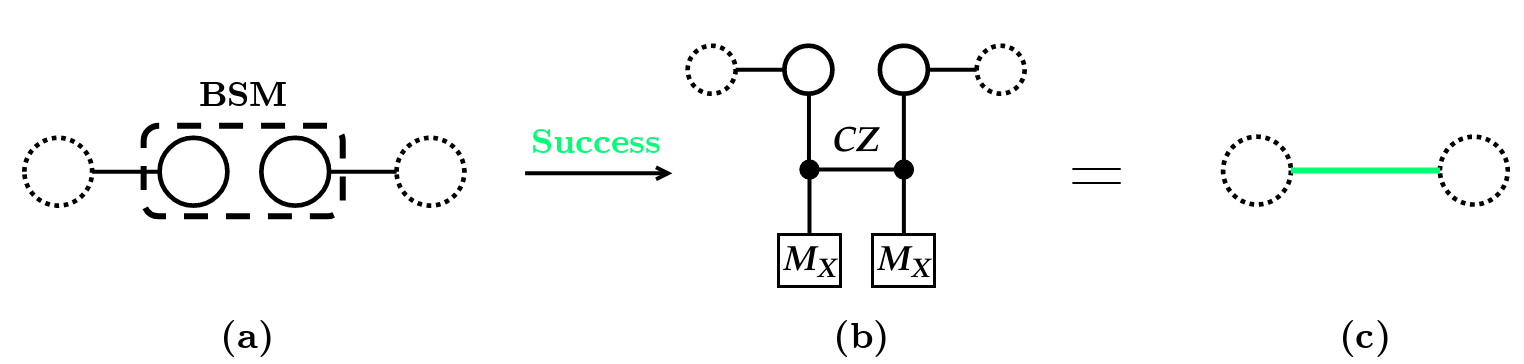
\includegraphics[width=\textwidth]{figures/background/BSM_combo.png}
    \caption{Entanglement swapping via a linear-optical \Gls{bsm}. \textbf{(a)} Two incoming photonic qubits from neighbouring resources interfere at a beamsplitter and are measured in the computational basis. Only two of the four Bell states are distinguishable, limiting the success probability to 50\% per attempt (Section~\ref{sec:bg:bellpairs}). \textbf{(b)} Graph-state representation of a successful \Gls{bsm}, equivalent to a $CZ$ gate followed by $X$-basis measurements ($M_X$) on the measured qubits. \textbf{(c)} The resulting edge (green) directly connects the two remaining qubits, establishing entanglement between the neighbouring resources.}
    \label{fig:bsm}
\end{figure}

\subsection{Backbone Selection Example}

Section~\ref{sec:bg:backbone} describes \emph{backbone selection}: at every \Gls{absa}, the first arm whose \Gls{bsm} succeeds is kept and every other arm at that hop is discarded, regardless of which arm that turns out to be. Figure~\ref{fig:app:backbone-selection} works through a concrete 3-hop chain to make this concrete: each \Gls{absa} independently keeps whichever of its arms first succeeds, and the surviving entanglement (bottom row) connects Alice to Bob only through the chain of kept arms, one hop at a time, regardless of which specific arm succeeded at each hop.

\begin{figure}[ht]
    \centering
    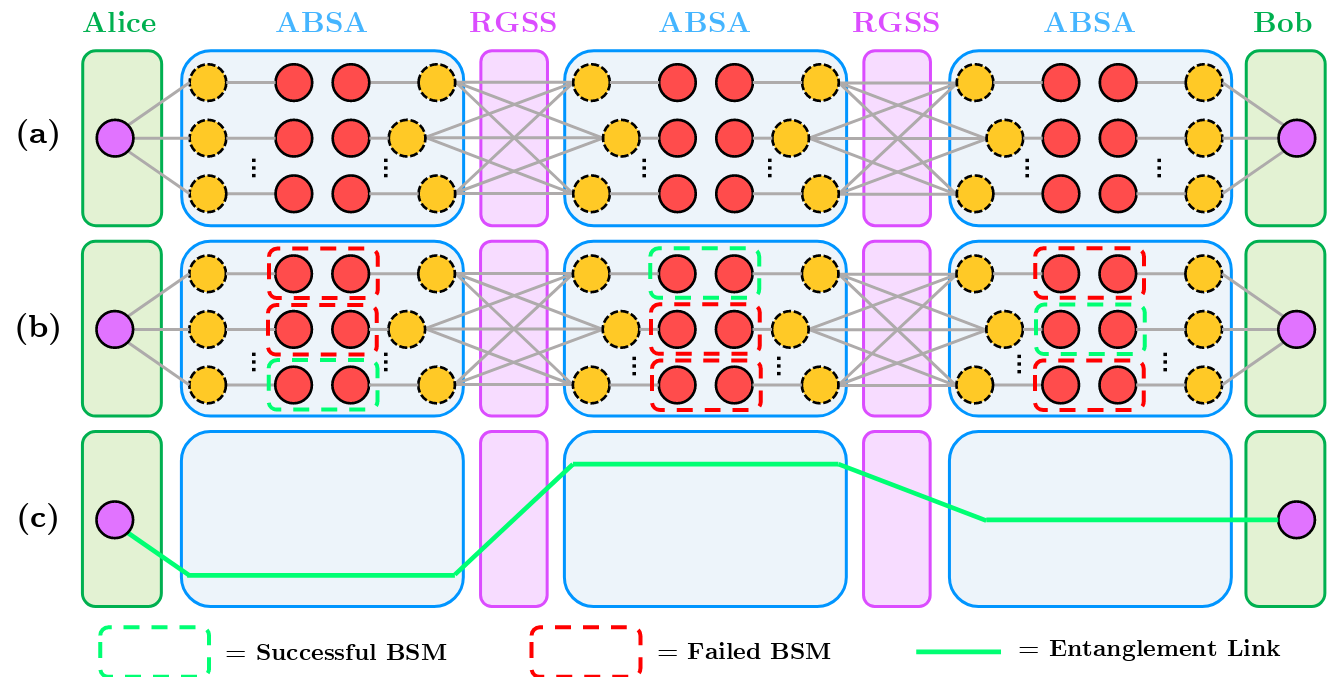
\includegraphics[width=\textwidth]{figures/background/ES_process.png}
    \caption{Backbone selection across a $N=3$-hop chain. \textbf{(a)} The network configuration before entanglement generation. Each \Gls{absa} initially holds outer/inner qubit pairs (red/yellow) for all provisioned arms connecting it to each of its two neighbouring stations. \textbf{(b)} At each \Gls{absa}, a \Gls{bsm} is attempted for every available arm. Multiple attempts may succeed, but once at least one successful \Gls{bsm} is obtained (green), one successful arm is selected and its corresponding inner qubits are retained, while the remaining arms are discarded. As this selection is performed independently at each \Gls{absa}, the retained arms need not correspond to the same arm index across the different hops. \textbf{(c)} The selected inner qubits form the backbone used to establish end-to-end entanglement. The resulting entanglement (green line) connects Alice to Bob through one retained arm at each hop, as described in Section~\ref{sec:bg:backbone}.}
    \label{fig:app:backbone-selection}
\end{figure}

\subsection{Purification Circuits}

Section~\ref{sec:bg:circuits} introduces the three purification circuits $\mathcal C_\mathrm{ZX}$, $\mathcal C_\mathrm{XZ}$, and $\mathcal C_\mathrm{YY}$ by the stabilizer each one measures. Figure~\ref{fig:app:circuits} below gives their circuit-level implementation.

% Circuit-level diagrams for the three purification circuits of
% Section~\ref{sec:bg:circuits}/\ref{sec:bg:purmath}. Each circuit acts on
% one retained and one measured qubit per party (Alice/Bob); the retained
% qubit survives as the purified output on success, the measured qubit is
% consumed by the local measurement whose outcome is compared between
% parties to determine success.

\begin{figure}[htbp]
    \centering

    \begin{subfigure}[t]{0.30\textwidth}
        \centering
        \begin{quantikz}[row sep=0.32cm, column sep=0.34cm]
            \lstick[2]{Alice} & \ctrl{1}  & \qw      & \qw      & \qw \\
                              & \targ{}   & \meter{} & \qw      & \qw \\
            \lstick[2]{Bob}   & \targ{}   & \qw      & \qw      & \qw \\
                              & \ctrl{-1} & \gate{H} & \meter{} & \qw
        \end{quantikz}
        \caption{$\mathcal C_\mathrm{ZX}$}
        \label{fig:app:circuit-zx}
    \end{subfigure}
    \hfill
    \begin{subfigure}[t]{0.30\textwidth}
        \centering
        \begin{quantikz}[row sep=0.32cm, column sep=0.34cm]
            \lstick[2]{Alice} & \targ{}   & \qw      & \qw      & \qw \\
                              & \ctrl{-1} & \gate{H} & \meter{} & \qw \\
            \lstick[2]{Bob}   & \ctrl{1}  & \qw      & \qw      & \qw \\
                              & \targ{}   & \meter{} & \qw      & \qw
        \end{quantikz}
        \caption{$\mathcal C_\mathrm{XZ}$}
        \label{fig:app:circuit-xz}
    \end{subfigure}
    \hfill
    \begin{subfigure}[t]{0.36\textwidth}
        \centering
        \begin{quantikz}[row sep=0.32cm, column sep=0.22cm]
            \lstick[2]{Alice} & \gate{H}         & \gate{S^\dagger} & \ctrl{1} & \gate{S} & \qw      & \qw \\
                              & \gate{H}         & \gate{S^\dagger} & \targ{}  & \gate{H} & \meter{} & \qw \\
            \lstick[2]{Bob}   & \gate{S^\dagger} & \ctrl{1}         & \gate{S} & \qw      & \qw      & \qw \\
                              & \gate{S^\dagger} & \targ{}          & \gate{H} & \meter{} & \qw      & \qw
        \end{quantikz}
        \caption{$\mathcal C_\mathrm{YY}$}
        \label{fig:app:circuit-yy}
    \end{subfigure}

    \caption{Circuit-level implementation of the three purification circuits introduced in Section~\ref{sec:bg:circuits}. Each circuit consumes two same-span resources, one held by Alice and one by Bob (top/bottom wire per party is the retained/measured qubit respectively), and produces one purified resource on the retained wires when the two parties' measurement outcomes agree. \textbf{(a)} $\mathcal C_\mathrm{ZX}$: Alice measures the $Z$-parity of her pair (\textsc{cnot} into her measured qubit, then measurement) while Bob measures the $X$-parity of his (\textsc{cnot} into his retained qubit, Hadamard, then measurement); success probability and output error vector in Eqs.~\eqref{eq:pzx} and~\eqref{eq:purzx}. \textbf{(b)} $\mathcal C_\mathrm{XZ}$: the same construction with Alice and Bob's local circuits exchanged, so Alice measures the $X$-parity and Bob the $Z$-parity (Eqs.~\eqref{eq:pxz}, \eqref{eq:purxz}). \textbf{(c)} $\mathcal C_\mathrm{YY}$: both parties apply a local $H$--$S^\dagger$ basis change before their \textsc{cnot}, so the compared parity is a joint $Y$-type stabilizer across all four qubits (Eqs.~\eqref{eq:pyy}, \eqref{eq:puryy}).}
    \label{fig:app:circuits}
\end{figure}

\clearpage

\section{Pseudocode and Concurrency Analysis}
\label{app:concurrency}

Section~\ref{sec:model:budget} defines the concurrency requirement $M(\Sigma)$ and its Sethi--Ullman recurrence~\cite{Sethi1970Generation}. This appendix gives the pseudocode implementing that recurrence as well as a complexity analysis.

The following pseudocode implements this recurrence. It assumes that the schedule is a binary tree and that each node exposes its children through $\texttt{children}(v)$.

\begin{algorithm}[ht]
\DontPrintSemicolon
\SetKwFunction{FRegReq}{RegisterRequirement}
\SetKwProg{Fn}{Function}{:}{}
\Fn{\FRegReq{$v$}}{
    \If{$v$ is \textup{\texttt{GenNode}}}{\Return $1$\;}
    \If{$v$ is \textup{\texttt{IdleNode}} or $v$ is \textup{\texttt{HeraldNode}}}{
        $c \gets \texttt{child}(v)$\;
        \Return \FRegReq{$c$}\;
    }
    $(c_1,c_2) \gets \texttt{children}(v)$\;
    $L \gets$ \FRegReq{$c_1$}\;
    $R \gets$ \FRegReq{$c_2$}\;
    \eIf{$L \neq R$}{\Return $\max(L,R)$\;}{\Return $L+1$\;}
}
\caption{Minimum concurrency requirement of a tree-shaped schedule}
\label{alg:concurrency}
\end{algorithm}

The procedure is evaluated recursively from the root, so every node is visited exactly once. Consequently, the computation takes $O(|T|)$ time and $O(h)$ auxiliary space for a tree of $|T|$ nodes and height $h$. The resulting value is thus the concurrency requirement $M(\Sigma)=\textsc{RegisterRequirement}(\mathrm{root}(T))$. The schedule satisfies the concurrency budget when $M(\Sigma)\leq M_{\max}$.
\chapter{Additional Experimental Results}
\label{app:results}

\TODO{for all tables that basically just restate in numbers some figure / chart already present in the main text, say that in their caption or introductory paragraphs i.e. "The values in this table correspond directly to those shown in Figure X in the main text." or somoething simialr}

\TODO{try to write sentences that don't feature the ';' as a way to seprarate stencens i prefer sentences that are shorter but clearer}

\TODO{overall, recheck that the different parts of the appendix are correctly linked back in the main text by checking the label/refs usage etc. check that the references are correctly pointing to the intended sections, figures, and tables in the main text.}

\TODO{the aim for this appendix should be to be a comprehensive repository of supplementary material that supports the main experimental results, providing additional numeric tables, extended figures, and detailed validation data. that means that anythign that isn't directly supporting the main experimental results should be excluded and removed. even if the reuslt seem interesting like 6/10 it should be removed. i only want the appendix to contain extra material like data that I couldn't fit in the main text, not be an extra chapter fitted in the appendix because I didn't have room in the 30 pages. remove anything thats not useful or not major}

\TOFIX{reread once finished}{This appendix collects material that supports Chapter~\ref{chap:experiments}, including extended numeric tables behind figures shown in the main text, supplementary figures for the search algorithms of Chapter~\ref{chap:algorithms}, and one additional optimality-scope result. Sections are grouped by what they support rather than one per table, and every table or figure below is referenced from the main-chapter passage that motivates it.}

\section{Experimental Parameters}
\label{app:params}

\TOFIX{maybe remove?}{Table~\ref{tab:params} summarizes every parameter varied anywhere in Chapter~\ref{chap:experiments}, alongside the reference value used whenever it is held fixed, and the section in which it is swept.}

\begin{table}[ht]
    \centering
    \small
    \begin{tabular}{p{5cm}lllp{3cm}}
        \toprule
        Parameter & Symbol & Reference ($\mathcal{N}_{\mathrm{ref}}$) & Swept ranges & Where varied \\
        \midrule
        Hop count & $N$ & 10 & 10--28 & Section~\ref{sec:exp:budget} \\
        Hop length & $\ell_i$ & 2~km & \{1, 2, 3, 4\}~km & Section~\ref{sec:exp:heterogeneous} \\
        Tree-encoding branching vector & $\vec b^{(i)}$ & $(16,14,1)$ & -- & not varied \\
        BSM arm count & $k_i$ & 18 & 6, 18 & Section~\ref{sec:exp:netgen} \\
        Inner-qubit error rates & $\{p_X^{\mathrm{in}},p_Z^{\mathrm{in}}\}_i$ & 0 & [0, $3\!\times\!10^{-3}$] & Section~\ref{sec:exp:netgen} \\
        Photon survival probability & $\eta_i$ & 0.912 & $10^{-0.2 \ell_i/10}$ & Section~\ref{sec:exp:heterogeneous} \\
        Outer-photon depolarizing rate & $e_d$ & 0.01 & $[0,\,0.01]$ & Section~\ref{sec:exp:edsweep} \\
        Memory dephasing rate & $\gamma$ & 0 & $[0,\,10^5]$ & Section~\ref{sec:exp:timing} \\
        Propagation speed & $c$ & $2\!\times\!10^5$~km/s & -- & not varied \\
        Emission delay & $\tau_{\mathrm{emit}}$ & 0 & $[10^{-4},\,1]$ & Section~\ref{sec:exp:timing} \\
        Generation-cost budget & $E_{\max}$ & 100 & 50--280 & Sections~\ref{sec:exp:headline}--\ref{sec:exp:budget} \\
        \bottomrule
    \end{tabular}

    \caption{Experimental parameters. The reference column gives the nominal value used unless a parameter is varied in the indicated experiment. All parameters not listed as varying follow the Integrating paper's~\cite{Benchasattabuse2025Integrating} reference configuration $\mathcal{N}_{\mathrm{ref}}$ (Section~\ref{sec:model:network}). The tree branching factor is not varied because it does not affect the objectives $F$, $C$, or $R$ introduced in Chapter~\ref{chap:model}. Uniform hop-length scaling likewise leaves relative schedule comparisons unchanged; heterogeneous hop lengths are considered separately in Section~\ref{sec:exp:heterogeneous}.}
    \label{tab:params}
\end{table}

\section{Extended Physics Validation}
\label{app:validation}

Section~\ref{sec:exp:validation} reports the evaluator's agreement with the Integrating paper's Fig.\,5~\cite{Benchasattabuse2025Integrating}, \TOFIX{rephrase}{similarly at $e_d=0.01$}. Table~\ref{tab:app:validation} and Figure~\ref{fig:app:validation} give the evaluator's fidelity output for the raw, heralded-pumping, and optimistic-pumping canonical schedules (Section~\ref{sec:bg:decoherence}) across the full $e_d \in [0, 0.01]$ used throughout Chapter~\ref{chap:experiments}.

\TOFIX{the source paper's fig 5 is exactly reproduced in fig:app:validation so idk why this paragraph seems to say there is only 2 published points...? make sure this paragraph phrases correctly that my evaluator reproduces exactly the values of the paper; verify previous paragraph and the conten of chapter 6 as well}{The source paper publishes numeric reference values at only two points on this grid, $e_d=0.000$ and $e_d=0.010$: approximately $\{1.000, 1.000, 1.000\}$ and $\{0.823, 0.917, 0.929\}$ respectively, for the same three schedules in the same order. The evaluator matches both to at least three significant figures, and to four at $e_d=0.010$ (the values already quoted in Section~\ref{sec:exp:validation}). \TOFIX{maybe rephrase?}{The other nine intermediate rows have no corresponding published value to compare against, since the source paper's own Fig.\,5 does not report numeric values between its two published points but are still featured here for completeness}.}

\TODO{highlight in bold the evaluator's output that matches the source paper's published values.}

\begin{table}[h]
    \centering\small
    \begin{tabular}{cccc}
        \hline
        $e_d$ & $F_{\text{raw}}$ & $F_{\text{baseline (heralded)}}$ & $F_{\text{flexible (optimistic)}}$ \\
        \hline
        0.000 & \textbf{1.0000} & \textbf{1.0000} & \textbf{1.0000} \\
        0.001 & 0.9803 & 0.9932 & 0.9933 \\
        0.002 & 0.9610 & 0.9861 & 0.9866 \\
        0.003 & 0.9422 & 0.9787 & 0.9799 \\
        0.004 & 0.9239 & 0.9710 & 0.9730 \\
        0.005 & 0.9061 & 0.9629 & 0.9661 \\
        0.006 & 0.8887 & 0.9544 & 0.9591 \\
        0.007 & 0.8717 & 0.9456 & 0.9519 \\
        0.008 & 0.8552 & 0.9364 & 0.9446 \\
        0.009 & 0.8391 & 0.9268 & 0.9372 \\
        0.010 & \textbf{0.8234} & \textbf{0.9168} & \textbf{0.9295} \\
        \hline
    \end{tabular}

    \caption{Evaluator-derived fidelity vs.\ $e_d$ for the three canonical schedules of Section~\ref{sec:bg:decoherence}, at $N=10$. Bold rows ($e_d=0.000$ and $e_d=0.010$) are the only two points with a published reference value to compare against (see text).}
    \label{tab:app:validation}
\end{table}

\begin{figure}[ht]
    \centering
    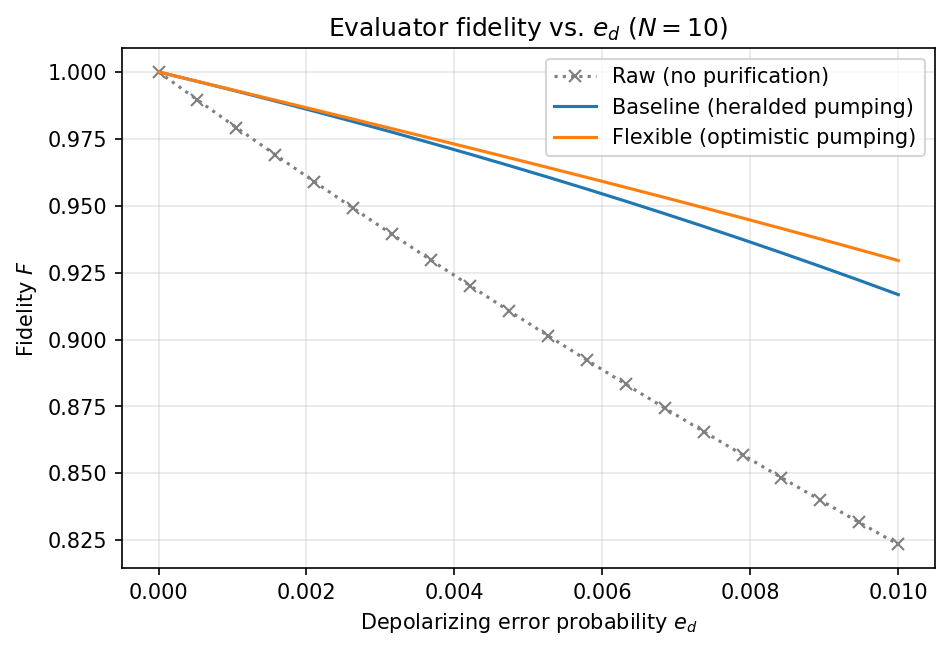
\includegraphics[width=0.7\textwidth]{figures/appendix/fidelity_vs_ed_validation.png}
    \caption{\TOFIX{add that this figure reproduces the source paper's Fig.\,5 exactly}{Evaluator fidelity vs.\ $e_d$ for the three canonical schedules of Table~\ref{tab:app:validation}, $N=10$. The raw chain degrades fastest; both pumping variants track closely, with the optimistic variant consistently slightly ahead of the heralded one over the whole range (Section~\ref{sec:disc:optimistic}).}}
    \label{fig:app:validation}
\end{figure}
\FloatBarrier

\section{Extended Network and Heterogeneity Comparisons}
\label{app:networks}

This section gives the full numeric backing for the two network-generalization experiments of Section~\ref{sec:exp:comparison}: uniformly applied non-ideal parameters (Section~\ref{sec:exp:netgen}) and per-hop heterogeneous networks (Section~\ref{sec:exp:heterogeneous}).

\subsection{Network Generalization Full Comparison}
\label{app:netgen}

Section~\ref{sec:exp:netgen} summarizes the network-generalization result. Table~\ref{tab:netgen} gives the full numeric comparison (cost, fidelity, and rate) behind Figure~\ref{fig:netgen}, across both tested \Gls{bsm} arm counts.

\begin{table}[h]
\centering
\caption{Optimizer versus the paper schedule under two non-ideal network configurations. Both use $N=10$, $e_d=0.01$, $E_{\max}=100$, $\gamma=0$, and non-zero inner-qubit error $p_X^{\mathrm{in}}=p_Z^{\mathrm{in}}=3\times10^{-3}$, unlike the source paper's idealized inner-qubit assumption. The configurations differ in the number of redundant \Gls{bsm} arms per hop. A schedule is feasible when $F\ge F_{\min}=0.9$.}
\label{tab:netgen}
\small
\begin{tabular}{llcccc}
\hline
Config & Schedule & $C$ & $F$ & Rate & Feasible \\
\hline
18 arms & Paper schedule & 100 & 0.67 & 103.18 & \textbf{no} \\
18 arms & Matched-cost & 100 & 0.90 & 25.31 & yes \\
18 arms & Budget-relaxed & 80 & 0.90 & 85.30 & yes \\
\hline
6 arms & Paper schedule & 100 & 0.87 & 871.55 & \textbf{no} \\
6 arms & Matched-cost & 100 & 0.93 & 681.56 & yes \\
6 arms & Budget-relaxed & 60 & 0.91 & 2096.91 & yes \\
\hline
\end{tabular}
\end{table}

\subsection{Heterogeneous Weak-Link Contrast}
\label{app:weaklink}

Section~\ref{sec:exp:heterogeneous} summarizes both the designed five-hop weak-link case and the 100-network random sample. Table~\ref{tab:weaklink} gives the full numeric comparison for the designed case: one hop with a $12\times$ higher inner-qubit error rate than its neighbours.

% Figure~\ref{fig:app:weaklink-allocation} shows how the two schedules allocate resources across that chain.

\begin{table}[ht]
    \centering
    \small
    \begin{tabular}{lcccc}
        \hline
        Schedule & $C$ & $F$ & Rate & Feasible \\
        \hline
        Best uniform link-level recipe & 40 & 0.88 & 1738.32 & \textbf{no} \\
        Optimizer's schedule & 38 & 0.90 & 1798.57 & yes \\
        \hline
    \end{tabular}

    \caption{Designed weak-link contrast for a heterogeneous $N=5$ network at $e_d=0.01$, $E_{\max}=50$, and $F_{\min}=0.9$. One hop has an inner-qubit error rate $12\times$ higher than its neighbours. The uniform link-level baseline uses the same purification configuration at every hop, whereas the optimizer may allocate resources differently across hops. A schedule is feasible when $F\ge F_{\min}$.}
    \label{tab:weaklink}
\end{table}

% \TODO{regenerate figure so that legend is both bigger font and without a border, below the figure}

% \begin{figure}[ht]
%     \centering
%     
\includegraphics[width=0.75\textwidth]{figures/results/weak_link_allocation.png}
%     \caption{Per-hop \texttt{GenNode} allocation for the optimizer's schedule and the best uniform link-level recipe, against the per-hop inner-qubit error rate, for the weak-link network of Table~\ref{tab:weaklink}. The optimizer spends less at hop 3 and reallocates the saved cost to the noisier hop 2, while the uniform recipe cannot vary its allocation across hops by construction.}
%     \label{fig:app:weaklink-allocation}
% \end{figure}
% \FloatBarrier

\TOFIX{rephrase, sounds too AI}{Figure~\ref{fig:app:heterogeneity} extends this single designed case to the full 100-network random sample}. It plots the optimizer's rate improvement over the best feasible uniform recipe, against each network's per-hop noise heterogeneity \TOFIX{what does this mean?}{(coefficient of variation of inner-qubit error rate across hops)}. Improvement is concentrated at \TOFIX{again too AI + what does it mean}{low-to-moderate heterogeneity}, where a single noisier hop still leaves room for the optimizer to reallocate resources profitably; the points sitting on the zero line are the ties noted in Section~\ref{sec:exp:heterogeneous}, \TOFIX{good but don't phrase with a not X but Y pattern like AI}{not cases where the optimizer underperforms}.


\TODO{regen figure, make legend's font bigger; rephrase the legends content maybe also color some points that are "performing" better? maybe not idk}

\begin{figure}[ht]
    \centering
    
\includegraphics[width=0.75\textwidth]{figures/results/random_sweep_improvement_vs_heterogeneity.png}
    \caption{Optimizer rate improvement over the best feasible uniform link-level recipe vs.\ per-hop noise heterogeneity, across the 100 random $N=6$ networks of Section~\ref{sec:exp:heterogeneous}. Points on the zero line are ties, not losses (Section~\ref{sec:disc:synthesis}).}
    \label{fig:app:heterogeneity}
\end{figure}
\FloatBarrier

\section{Extended Cost-Quality and Optimality Results}
\label{app:costquality}

\subsection{Alternative Objectives, Full Comparison}
\label{app:objectives}

Section~\ref{sec:exp:objectives} summarizes the objective-substitution result; Table~\ref{tab:app:objectives} gives the full five-objective comparison it draws from, at $N=10$ and $e_d=0.01$.

\begin{table}[ht]
    \centering
    \small
    \begin{tabular}{lccc}
        \hline
        Objective & $C$ & $F$ & Rate \\
        \hline
        Maximize rate & 60 & 0.9063 & 6195.95 \\
        Maximize fidelity, paper-rate floor & 80 & 0.9351 & 4804.58 \\
        Maximize fidelity, matched-rate floor & 80 & 0.9351 & 4804.58 \\
        Minimize cost, $F \ge 0.9$ only & 60 & --- & 1239.19 \\
        Minimize cost, $F \ge 0.9$ and $R \ge 4804.58$ & 60 & --- & 6195.95 \\
        \hline
    \end{tabular}

    \caption{Objective-substitution comparison at $N=10$, $e_d=0.01$: five objective definitions with no change to the search algorithm.}
    \label{tab:app:objectives}
\end{table}

\section{Search Algorithm Diagnostics}
\label{app:searchalgos}

\TODO{goal of this section is to justify the chosen beam width value and that beam search scales comparably to the exact dynamic program once same-span pumping is enabled. focus on that}

\TOFIX{which? does it mean instead "the following observations/diagnostics"}{These diagnostics} justify two implementation choices used throughout Chapter~\ref{chap:experiments}: the default beam width $w_{\mathrm{beam}}=25$ (Section~\ref{sec:alg:beam}) and the claim that beam search scales comparably to the exact dynamic program once same-span pumping is enabled (Section~\ref{sec:alg:pumping}).

\TOFIX{unclear and confused}{Figure~\ref{fig:app:beamwidth} shows why $w_\text{beam}=25$ was chosen as the default beam width: at $N=10$, wall-clock search time grows mildly up to a beam width of about 16 and then sharply beyond it, while the best rate found is already flat across the entire tested range, so widening the beam past 25 buys no further quality improvement at this configuration. Separately, at $N=6$, where the exact dynamic program (Section~\ref{sec:alg:dp}) remains tractable, beam search matches its exact optimum at every beam width tested from 1 to 32, with zero gap throughout -- confirming that this determinism holds even at the smallest beam widths, not only at the default.}

\TODO{regenerate figure to fix position and size of legend (to be bigger and not positioned middle left but top left in a box with larger font.) the blue line is also literally just a straight line on the graph so it looks weird. overall that graph is unreadable with 3 different axes.}

\begin{figure}[ht]
    \centering
    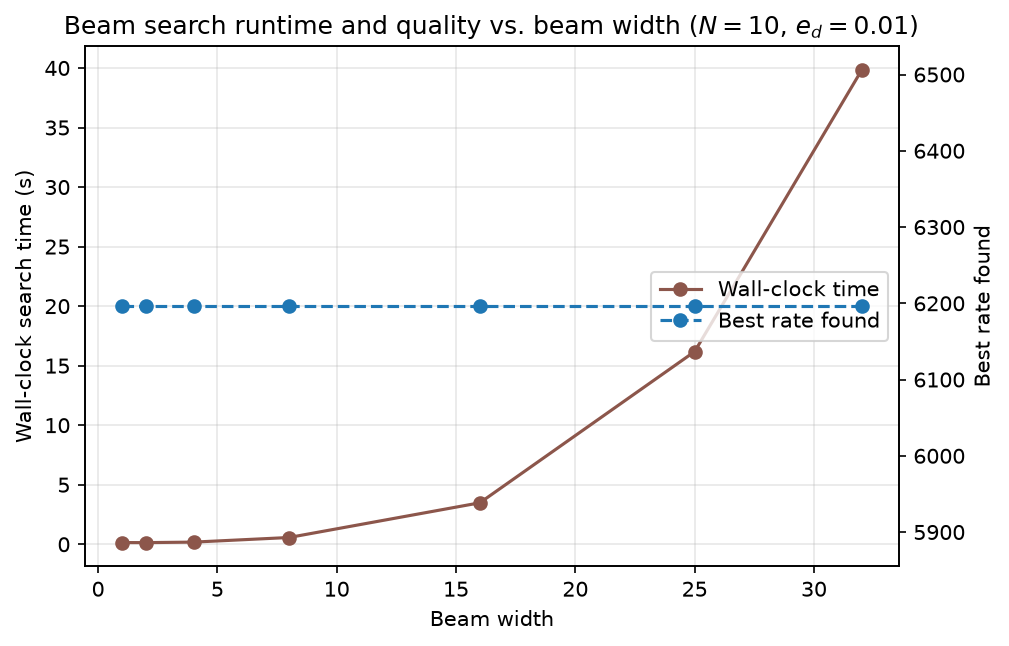
\includegraphics[width=0.75\textwidth]{figures/appendix/runtime_and_quality_vs_beam_width.png}
    \caption{Beam search wall-clock time and best rate found vs.\ beam width, at $N=10$, $e_d=0.01$.}
    \label{fig:app:beamwidth}
\end{figure}
\FloatBarrier

Figure~\ref{fig:app:runtimen} extends the runtime comparison of Table~\ref{tab:benchmarks} (Section~\ref{app:runtime}) to every tested $N$: both the exact dynamic program and the beam search scale similarly with $N$ once the same-span pumping move is enabled, with the beam search consistently the faster of the two.

\begin{figure}[H]
    \centering
    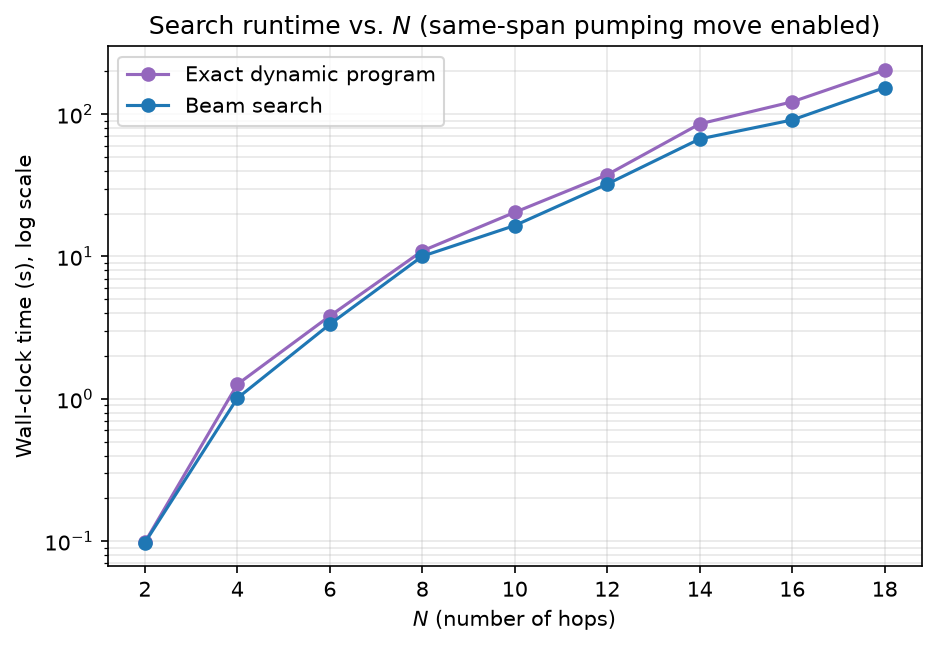
\includegraphics[width=0.75\textwidth]{figures/appendix/runtime_vs_n_pumping.png}
    \caption{Search wall-clock time vs.\ $N$ for the exact dynamic program and the beam search, same-span pumping move enabled throughout.}
    \label{fig:app:runtimen}
\end{figure}
\FloatBarrier

\subsection{Concurrent Branch Budget ($M_{\max}$)}
\label{app:mmax}

\TODO{move this subsection in appendix A below the pseudo code and make it shorter + make sure it doesn't repeat the content already discussed in that appendix A}

Section~\ref{sec:model:scope} notes that $M_{\max}$, the number of concurrently open branches (Section~\ref{sec:model:budget}), is computed exactly for a given schedule but is not used to prune the search itself. Table~\ref{tab:app:mmax} gives $M(\Sigma)$ for the fixed schedule families and the optimizer's own budget-relaxed best schedule across $N=2$ to $N=18$ at $e_d=0.01$: no family shows $M(\Sigma)$ growing with $N$, since the register-allocation bound (Section~\ref{sec:model:budget}) is governed by \Gls{dag} depth and branching shape rather than hop count. Bisecting $m_{\max}$ downward from the unconstrained optimum at $N=10$, $E_{\max}=100$ shows that the budget-relaxed optimum ($M=4$) remains selectable down to $m_{\max}=4$, but no candidate in the beam-searched frontier clears both the rate objective and $m_{\max}=3$, at which point $M_{\max}$ becomes the actual binding constraint rather than $E_{\max}$ or $F_{\min}$.

\begin{table}[h]
    \centering
    \small
    \begin{tabular}{cccc}
        \hline
        $N$ & Raw chain & Heralded end-node pumping & Optimizer (budget-relaxed) \\
        \hline
        2  & 3 & 4 & 3 \\
        4  & 3 & 4 & 4 \\
        6  & 3 & 4 & 4 \\
        8  & 3 & 4 & 4 \\
        10 & 3 & 4 & 4 \\
        14 & 3 & 4 & 4 \\
        18 & 3 & 4 & 5 \\
        \hline
    \end{tabular}

    \caption{$M(\Sigma)$ vs.\ $N$ for the fixed schedule families and the budget-relaxed optimum, $e_d=0.01$.}
    \label{tab:app:mmax}
\end{table}

\subsection{Runtime Benchmarks}
\label{app:runtime}

Table~\ref{tab:benchmarks} gives the wall-clock time and returned score underlying Figure~\ref{fig:app:runtimen} and the beam-width discussion above, at representative chain lengths, together with the two cases (footnoted in the table) where the pumping-enabled exact dynamic program is not a strict upper bound on beam search (Section~\ref{sec:alg:pumping}).

\begin{table}[ht]
    \centering
    \small
    \begin{tabular}{rrllrr}
        \toprule
        $N$ & $E_{\max}$ & Exact DP (s) & Beam search (s) & Exact DP score & Beam search score \\
        \midrule
        2  & 20  & 0.10 & 0.10 & 50\,000 & 50\,000 \\
        6  & 60  & 3.82 & 3.34 & 14\,372\textsuperscript{$\ddagger$} & 15\,391 \\
        10 & 100 & 20.43 & 16.50 & 6\,196 & 6\,196 \\
        14 & 140 & 85.37 & 66.93 & 3\,394 & 3\,394 \\
        18 & 180 & 203.68\textsuperscript{$\dagger$} & 153.52 & $-\infty$ & 1\,214 \\
        \bottomrule
    \end{tabular}

    \caption{Wall-clock runtime and returned score for the exact dynamic program and beam search at representative chain lengths. Runs use $E_{\max}=10N$, $F_{\min}=0.9$, beam width $w_{\mathrm{beam}}=25$, same-span pumping enabled (Section~\ref{sec:alg:pumping}), a 300~s timeout, and a 3~GiB memory limit. The score is the value of the active objective; here, it is the returned schedule rate $R(\Sigma)$. \textsuperscript{$\dagger$}At $N=18$, the exact dynamic program completes within the timeout but finds no feasible candidate, while beam search returns a feasible one. \textsuperscript{$\ddagger$}At $N=6$, beam search returns a higher score than the exact dynamic program. These cases arise because same-span pumping is itself beam-limited, so the pumping-enabled exact dynamic program is not guaranteed to upper-bound beam search (Section~\ref{sec:alg:pumping}).}
    \label{tab:benchmarks}
\end{table}

\section{Timing Sensitivity, Full Sweeps}
\label{app:timing}

% Source: outputs/sweep_gamma_and_tau_emit/README.md

Section~\ref{sec:exp:timing} summarizes the effect of memory dephasing and generation latency on schedule rate and fidelity; Figure~\ref{fig:timing} gives both sweeps in full, at $N=10$ and $e_d=0.01$.

\paragraph{Memory dephasing ($\gamma$)}

Sweeping $\gamma$ from 0 to $10^5$ leaves the raw chain and paper schedule's fidelity unchanged across the tested range: neither contains a resource that waits for another branch to become ready, so the simulated execution introduces no additional memory-decoherence interval for these schedules. By contrast, heralded end-node pumping falls from $F=0.92$ at $\gamma=0$ to $F=0.25$, the maximally mixed limit, at $\gamma=10^5$, because its sacrificial copies remain stored while each round-trip heralding delay is incurred. The schedules selected by the optimizer remain flat across the tested values of $\gamma$; this does not mean memory dephasing is generally harmless, only that the search favours optimistic schedules in which the relevant intermediate heralding delays are deferred, avoiding the specific waiting pattern that causes the collapse of the heralded pumping schedule (Section~\ref{sec:disc:optimistic}).

\paragraph{Generation latency ($\tau_{\mathrm{emit}}$)}

Sweeping $\tau_{\mathrm{emit}}$ at $\gamma=0$ reduces the rate monotonically for every schedule. The relative rate loss is largest for the optimistic pumping family, whose baseline latency is approximately $1\times L/c$, and smallest for heralded end-node pumping, whose baseline latency is approximately $9\times L/c$: a schedule that already has a larger fixed latency is proportionally less affected by the same additional per-photon generation delay. The two schedules cross near $\tau_{\mathrm{emit}}\approx0.01$; above this value, the larger fixed latency of heralded pumping makes it less sensitive, in relative terms, to further increases in generation latency.

\begin{figure*}[ht]
    \centering
    \begin{subfigure}[b]{0.48\textwidth}
        \centering
        
\includegraphics[width=\textwidth]{figures/results/gamma_fidelity.png}
        \caption{Fidelity vs.\ $\gamma$}
    \end{subfigure}
    \hfill
    \begin{subfigure}[b]{0.48\textwidth}
        \centering
        
\includegraphics[width=\textwidth]{figures/results/tau_emit_rate.png}
        \caption{Rate vs.\ $\tau_{\mathrm{emit}}$ (log-log)}
    \end{subfigure}
    \caption{Timing sensitivity of the raw chain, the paper schedule, and heralded end-node pumping, at $N=10$ and $e_d=0.01$.}
    \label{fig:timing}
\end{figure*}
\FloatBarrier

\section{Schedule DAGs of Selected Optima}
\label{app:dags}

The schedules found in Chapter~\ref{chap:experiments}, such as the budget-relaxed optimum at $N=10$ (Section~\ref{sec:exp:headline}), are automatically constructed \Glspl{dag} with 50 to 100 \texttt{GenNode} leaves and several hundred nodes once every backbone and purification step is counted. Rendered at a scale where individual node labels stay legible, such a diagram does not fit within a single printed page: the same rendering tooling used for the worked $N=2$ example of Figure~\ref{fig:model:dag-example} produces images several thousand pixels wide once applied to these larger, automatically-constructed schedules, since node count (not page size) is the limiting factor.

Reproducing one of these diagrams here at a reduced scale would not add information beyond what Chapter~\ref{chap:experiments}'s tables and the Pareto frontier of Figure~\ref{fig:pareto} already convey, namely each schedule's cost, fidelity, rate, and overall shape family (e.g.\ end-node pumping vs.\ a span-partition structure), while making every individual node illegible. Figure~\ref{fig:model:dag-example} therefore remains the representative illustration of the \Gls{dag} representation itself, at a size deliberately chosen to exercise every node type from Section~\ref{sec:model:dag} while staying legible; the full artifacts for every optimum discussed in this thesis are reproducible directly from the search calls and parameters documented in Chapter~\ref{chap:algorithms} and Table~\ref{tab:params}.

\end{document}